\documentclass[preprint,12pt,authoryear]{elsarticle}
\usepackage{amsmath,amssymb,amsthm}
\usepackage{booktabs}
\usepackage{graphicx}
\usepackage{xcolor}
\usepackage{adjustbox}
\usepackage{hyperref}
\usepackage{algorithm}
\usepackage{algpseudocode}
\usepackage{tikz}
\usetikzlibrary{arrows.meta,positioning}
\usepackage[section]{placeins}
\begin{document}
\begin{frontmatter}
\title{Examination before attraction: lifelong affinities and detection-adjusted item appeal for recommendation under randomised exposure}
\author{Anonymous}
\begin{abstract}
Logs written by a deployed policy answer only indirectly how users respond to randomly placed items. We propose two log-only signals. LEAF summarises each user's long-term click rate on tags, authors and music of videos outside the test pool, conditional on exposure, and passes these affinities to a graph recommender. DAX models each logged impression as an examination, depending on the user and scenario, followed by an attraction, depending on the item. On KuaiRand-27K, with random insertions for validation and testing, the combined model reaches an nDCG@10 of 0.4854, against 0.4634 for a propensity-weighted LightGCN (PW-LightGCN), our unpublished baseline. The margins over PW-LightGCN and over DIN with DAX are significant but narrow. The PW-LightGCN margin is unchanged under two further training seeds, and the DIN margin is larger under matched capacity and those seeds, all significant at split level. DAX increases per-user nDCG@10 on all six backbones, and at split level on five. Correcting click rates for examination makes the item score useful: removing the examination model significantly lowers the gain, and alone DAX does no better than popularity. Shuffling lifelong statistics across users, or permuting attractiveness across items, removes the gain. The evidence comes from one platform.

\end{abstract}
\begin{keyword}
recommender systems \sep exposure bias \sep click models \sep lifelong user behaviour \sep randomised exposure \sep graph collaborative filtering
\end{keyword}
\end{frontmatter}
\section{Introduction}
\label{sec:intro}

A recommender on a short-video platform is trained on the platform's own logs. These logs record which videos the
production recommender, the \emph{policy}, chose to show to which users, in which part of the application, and whether
the users clicked. A model fitted to such a record learns how the audiences selected by the policy responded, and a
model that ranks well on a held-out part of the same record is partly rewarded for reproducing the policy. Many decisions
of a platform depend on a different question: how would a user respond to a video that the policy would not have chosen
for that user? This question arises whenever the platform explores new items, promotes content beyond its usual audience,
or changes its recommender. Some platforms measure it directly by occasionally filling a feed slot with a video drawn
uniformly at random from a pool. The KuaiRand data \citep{gao2022kuairand} contain such random insertions for thousands of
users, and they make it possible to evaluate a recommender on items that reach users regardless of what the policy
predicted.

\paragraph{Why logged clicks mislead} Consider a viewer who regularly watches cooking videos, and a short cooking clip by a
little-known author that is inserted into her feed at random. Two facts make this clip hard to rank from the policy log.
First, the clip's logged click rate may be low for reasons that have nothing to do with its appeal. If the policy showed it
mostly to users who rarely click anything, or in a part of the application where people scroll quickly, many of its
non-clicks come from viewers who never really looked at it. An item can stay unclicked because it was never examined, not
because it is unappealing. Second, the viewer may never have been shown any video from the random pool, so the policy log
says little about her taste for this clip. What she likes is recorded elsewhere, in her long history on the millions of
videos outside the pool, but simply counting how many cooking videos she was shown would measure the policy's choices rather
than her preferences.

\paragraph{The gap} Existing work addresses each of these problems in a different setting. Lifelong behaviour models such as
DIN, SIM and TWIN \citep{zhou2018din,pi2020sim,chang2023twin} exploit long user histories, but they are trained and evaluated on
policy logs, where history and target share item identifiers. Debiasing methods reweight the training loss by estimated
exposure propensities \citep{saito2020unbiased,joachims2017unbiased} or model exposure as a latent variable
\citep{liang2016exposure}; they still treat a shown-but-unclicked item as evidence against the item, whatever the attention of the
viewer. Click models for web search \citep{richardson2007predicting,craswell2008cascade,chuklin2015clickmodels} separate the
examination of a result from its attractiveness, but examination there depends on the rank position in a result list, which a
single feed slot does not have. Methods that learn from a small uniformly exposed sample \citep{chen2021autodebias} use the very data
that should be reserved for evaluation. We found no method that estimates, from the policy log alone, how a randomly chosen user
would respond to an item, and that is evaluated on randomly inserted items.

\paragraph{Our approach} We propose two signals, one for each side of the mismatch, both computed from data that a platform logs
anyway.
\begin{itemize}
\item \emph{A user's long-term behaviour outside the evaluated pool says what the user likes.} LEAF (lifelong exposure-conditional
  affinities) computes, for every user and every tag, author and music track, how much more often the user clicked videos with that
  key \emph{when they were shown} than her other videos, together with how familiar she is with the key. Because the statistics are
  conditional on exposure, they describe the user's response rather than the policy's choices. Content keys carry them from videos
  outside the pool to the candidates. LEAF-LGN adds these affinities to the graph recommender LightGCN \citep{he2020lightgcn}.
\item \emph{A non-click should count against an item only if the item was examined.} DAX (detection-adjusted attractiveness) models
  each logged impression as an examination, whose probability depends on the user and on the scenario, followed by an attraction,
  whose probability depends on the item. The idea comes from two fields. Occupancy models in ecology \citep{mackenzie2002occupancy}
  separate whether a species is present at a site from whether a survey detects it, and click models in information retrieval separate
  whether a result is examined from whether it attracts a click. In DAX an impression plays the role of a survey and a click the role
  of a detection. The item attractiveness is estimated by expectation-maximisation, with shrinkage towards the mean of the item's tag,
  and is added to any trained recommender with a weight chosen on validation users.
\end{itemize}
The combined model, LEAF-LGN+DAX, ranks the randomly inserted candidates with the LEAF-LGN score corrected by the attractiveness
that DAX assigns to each candidate.

\paragraph{Evaluation design} The evaluation is built so that the random insertions are never seen during training. All
training signals, including the lifelong statistics and the DAX fit, are computed from events before the start of the random
period. The random insertions are used only to select hyperparameters on one group of users and to measure accuracy on another,
over five user-level splits. Every comparison is tested twice, with a paired test over users and with a split-level test that
accounts for the shared training run, and both are corrected for multiple comparisons. The baselines include graph recommenders, a
debiased graph recommender, a closed-form recommender and two lifelong deep models, each also given the DAX module. Permutation
controls check that the gains depend on the users' own histories and on item-specific attractiveness.

\paragraph{Main findings} On KuaiRand-27K, LEAF-LGN+DAX reaches an nDCG@10 of 0.4854, against 0.4634 for the strongest debiased
graph baseline, a propensity-weighted LightGCN that we describe in
\ref{app:qp}, and 0.4733 for the same baseline with DAX added. It is ahead of each of the nine baselines of the main
comparison on both tests after Holm correction, although two of these comparisons are borderline on the split-level test. Adding DAX improves
each of six backbones on the per-user test. Permuting the attractiveness across items removes the DAX gain, and shuffling the
lifelong histories across users removes the gain of the lifelong channels. On the smaller KuaiRand-1K release, the advantage
over the debiased graph baseline, with and without DAX, is repeated.

\paragraph{Contributions}
\begin{itemize}
\item We formulate recommendation for randomly inserted items as a learning problem in which only the policy log may be used for
  training, and show on KuaiRand that the remaining accuracy headroom of a strong graph recommender lies in item-level appeal, not in
  temporal drift.
\item We propose LEAF, exposure-conditional affinities computed from each user's history outside the evaluated pool and transferred
  through content keys, and LEAF-LGN, which learns how much each affinity counts inside a graph recommender.
\item We propose DAX, a generative model of logged clicks that separates user and scenario examination from item attractiveness,
  borrowing the detection idea of occupancy models and click models, with an expectation-maximisation estimator and priors that pool
  information over tags and over each user's lifelong history.
\item We provide an evaluation in which the random insertions are reserved for selection and testing, with split-level tests,
  baselines that receive the same DAX module, and permutation controls for both signals.
\end{itemize}
We do not claim that DAX recovers an unbiased or causally identified item quality, and all evidence comes from one platform family
(Section~\ref{sec:limits}).

\paragraph{Outline} Section~\ref{sec:related} relates the work to lifelong behaviour models, click models, exposure-aware
recommendation, occupancy and small-area estimation, and debiased graph recommenders. Section~\ref{sec:method} defines the problem,
LEAF, DAX and their combination. Section~\ref{sec:protocol} describes the data, the temporal protocol and the statistical tests.
Section~\ref{sec:results} reports the results, Section~\ref{sec:discussion} discusses them, Section~\ref{sec:limits} states the
limitations and Section~\ref{sec:conclusion} concludes.

\section{Related work}
\label{sec:related}

\paragraph{Lifelong behaviour models} SIM \citep{pi2020sim} selects behaviours from a lifelong sequence that match the category of
the target, and TWIN \citep{chang2023twin} applies two-step target attention over a lifelong sequence on the Kuaishou platform,
which belongs to the platform family of KuaiRand. Both learn from policy logs and rely on item identifiers that the history shares
with the target. LEAF uses exposure-conditional statistics, transfers them to a pool disjoint from the history through content keys,
and is evaluated on random insertions. DIN \citep{zhou2018din} and SIM-hard are baselines here; TWIN is not.

\paragraph{Click models and examination} A click model explains a click as the product of an examination and a judgement about the
item. The position-based model \citep{richardson2007predicting}, the cascade model \citep{craswell2008cascade} and the monograph of
\citet{chuklin2015clickmodels} make examination depend on the rank of the item, and the dynamic Bayesian network
\citep{chapelle2009dbn} adds a satisfaction state. DAX has neither a position term nor a satisfaction state. Its examination depends
on the user and the scenario, and its target is item appeal under uniform insertion.

\paragraph{Exposure-aware and debiased recommendation} Impression-aware recommenders use shown but unclicked items as evidence
\citep{perezmaurera2025iars}. ExpoMF \citep{liang2016exposure} treats exposure as a latent variable fitted by EM. Inverse-propensity
estimators for missing-not-at-random feedback \citep{saito2020unbiased,joachims2017unbiased,schnabel2016} weight the loss, and doubly
robust estimators \citep{wang2019drjl,guo2021mrdr} add an imputation model. IPS-MF, DR-JL and MRDR, together with the graph model NAVIP
\citep{kim2022navip}, are published baselines here. AutoDebias \citep{chen2021autodebias} learns its debiasing parameters from a small
uniform sample, which the present protocol does not allow. DAX is a generative model of examination and appeal fitted by EM. The
estimators above weight a loss or use impressions as negatives or features.

\paragraph{Occupancy and small-area estimation} Occupancy models separate the presence of a species from its detection in repeated
surveys \citep{mackenzie2002occupancy}, so a site can be occupied and still yield no detection. Small-area estimation shrinks noisy
direct estimates towards a regression on area covariates \citep{fay1979smallarea}. The likelihood of DAX has the same structure as
the occupancy model: an impression plays the role of a survey, a click the role of a detection, and the attractiveness of an item
the role of presence. Its estimand, however, is appeal under a uniform audience. We are not aware of a recommendation paper that
uses this likelihood on a policy log.

\paragraph{Evaluation under randomised exposure} KuaiRand \citep{gao2022kuairand} ships randomly exposed videos in its feed logs, and
several recent papers use them for evaluation: propensity calibration \citep{hu2025uncertainty}, debiasing of watch-time signals
\citep{zhao2023d2co}, the reliability of the evaluation of debiasing methods \citep{wang2025debiasunreliable}, and category means in
logs with random insertions \citep{zhang2026categorymeans}. To our knowledge none of them uses the out-of-pool history of each user in
the random test, which is the source of the LEAF channels here.

\paragraph{Graph recommenders} The backbones are LightGCN \citep{he2020lightgcn}, EASE \citep{steck2019ease} and the r-AdjNorm
normalisation \citep{zhao2022radjnorm}. Debiasing work for graph recommenders acts on propagation or on popularity
\citep{kim2022navip,zhang2021pda}, and uses neither impressions nor lifelong data.

The contribution is the combination rather than any single ingredient. Each ingredient has a precedent: lifelong behaviour
statistics, examination multiplied by attractiveness, and Beta shrinkage towards a group mean. We are not aware of a work that
combines lifelong channels built from other pools, examination factors for the user and the scenario, and randomly inserted items as
the test target. Table~\ref{tab:positioning} in Appendix E lists the closest works.

\section{Method}
\label{sec:method}

This section first states the ranking problem and the data available to solve it
(Section~\ref{sec:method-notation}). It then describes the two signals that we add to a collaborative
recommender. LEAF summarises what a user's long-term behaviour on other videos says about the content of a
candidate video (Sections~\ref{sec:method-leaf} and~\ref{sec:method-leaflgn}). DAX estimates how attractive a video
is once it has actually been looked at, by separating examination from attraction in the logged clicks
(Section~\ref{sec:method-dax}). Section~\ref{sec:method-combine} explains how the two are combined, and
Section~\ref{sec:method-identify} states what the estimated attractiveness does and does not measure.
Detailed settings and the search grids are given in \ref{app:impl} and \ref{app:grids}.

Throughout the section we use one running example: a viewer who regularly watches cooking videos, and a short
cooking clip by a little-known author that the evaluation inserts into her feed at random.

\subsection{Problem setting and notation}
\label{sec:method-notation}

\paragraph{Users, items, scenarios and the cut-off} Let $\mathcal U$ be the set of users, with $m=|\mathcal U|$.
Let $\mathcal I$ be the pool of videos from which the random insertions are drawn; it is the set of videos that
appear in the random-exposure log. A platform shows videos in several scenarios, which are the tabs of the application
in which a video is placed. We write $\mathcal T$ for the set of scenarios, of which there are fifteen. The random
insertions fall almost entirely in one scenario, which we call $t=1$, and the scenario factor of
Section~\ref{sec:method-dax} is normalised to this scenario. A time $T_0$, the cut-off, separates the data used for learning
from the data used for evaluation.

\paragraph{Three logs} We use three sources of data, all of which a platform records routinely.
\begin{enumerate}
\item The \emph{policy log} $\mathcal D$ is the set of impressions of pool videos before $T_0$, as chosen by the production
  recommender. An impression $r\in\mathcal D$ records a user $u_r$, an item $i_r\in\mathcal I$, a scenario
  $t_r\in\mathcal T$ and a click indicator $y_r\in\{0,1\}$, which equals one when the user clicked the video. For a pair
  $(u,i)$ we write $X_{ui}=1$ if $u$ clicked $i$ at least once before $T_0$, and $N_{ui}=1$ if $u$ was shown $i$ before $T_0$
  but never clicked it.
\item The \emph{lifelong log} of a user is the set of that user's impressions before $T_0$ on videos \emph{outside} the
  pool $\mathcal I$, with their clicks. On a large platform this history is far longer than the user's history on the
  pool.
\item The \emph{random-exposure log} contains the impressions after $T_0$ in which a feed slot was filled with a video
  drawn uniformly at random from $\mathcal I$. It supplies the candidate lists and labels described below, and nothing else.
\end{enumerate}
Figure~\ref{fig:timeline} shows how the three logs are placed in time.

\paragraph{Candidate lists and labels} For a user $u$, the candidate list $C_u\subseteq\mathcal I$ is the set of pool
videos that were inserted at random for $u$ after $T_0$, with every pair that $u$ was shown in the policy log before $T_0$
removed. The label of a candidate is the click indicator of its random impression, so a candidate is relevant when the
user clicked it. The users are divided into a validation part and a test part (Section~\ref{sec:protocol-splits}). The
candidate lists and labels of the validation users select the configuration, and those of the test users measure accuracy.
A user without a click among the candidates has no defined nDCG@10 and is not scored.

\begin{figure}[tbp]
\centering
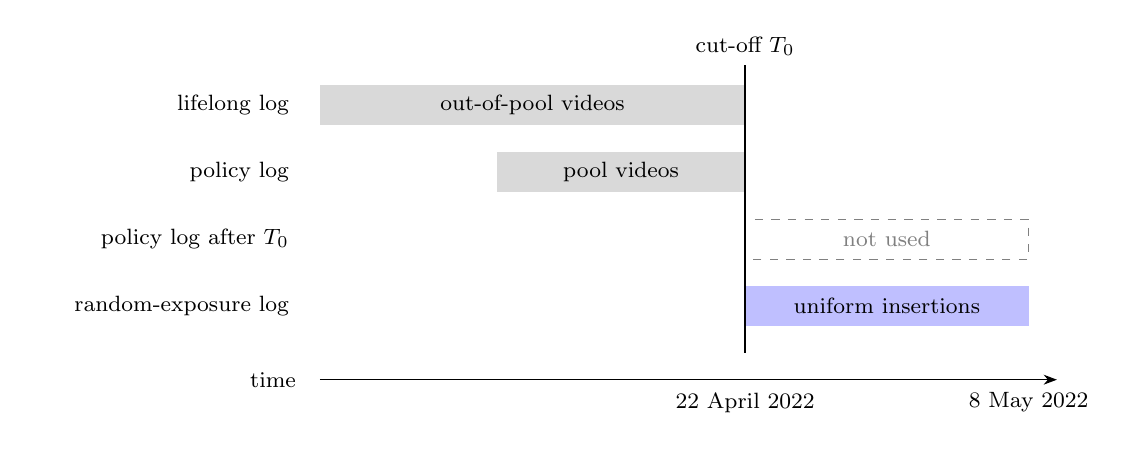
\begin{tikzpicture}[x=0.9cm,y=0.85cm,every node/.style={font=\footnotesize}]
  \node[anchor=east,align=right,text width=3.2cm] at (-0.3,2) {lifelong log};
  \node[anchor=east,align=right,text width=3.2cm] at (-0.3,1) {policy log};
  \node[anchor=east,align=right,text width=3.2cm] at (-0.3,0) {policy log after $T_0$};
  \node[anchor=east,align=right,text width=3.2cm] at (-0.3,-1) {random-exposure log};
  \fill[gray!30] (0,1.7) rectangle (6,2.3);
  \node at (3,2) {out-of-pool videos};
  \fill[gray!30] (2.5,0.7) rectangle (6,1.3);
  \node at (4.25,1) {pool videos};
  \draw[dashed,gray] (6,-0.3) rectangle (10,0.3);
  \node[gray] at (8,0) {not used};
  \fill[blue!25] (6,-1.3) rectangle (10,-0.7);
  \node at (8,-1) {uniform insertions};
  \draw[thick] (6,-1.7) -- (6,2.6);
  \node[anchor=south] at (6,2.6) {cut-off $T_0$};
  \draw[-{Stealth}] (0,-2.1) -- (10.4,-2.1);
  \node[anchor=east] at (-0.2,-2.1) {time};
  \node[below] at (6,-2.15) {22 April 2022};
  \node[below] at (10,-2.15) {8 May 2022};
\end{tikzpicture}
\caption{The three logs in time. The lifelong log and the policy log end at the cut-off $T_0$, and the random-exposure log
  starts there. Only the random-exposure log supplies candidates and labels, and only to the validation and test users. The
  policy log after the cut-off is drawn for completeness and is not used. The bars are schematic and not to scale.}
\label{fig:timeline}
\end{figure}

\paragraph{Content keys} Each video carries content keys from three families,
$\mathcal K=\{\mathrm{tag},\mathrm{author},\mathrm{music}\}$. For a family $k\in\mathcal K$, $v_k(i)$ denotes the key value
of video $i$ (its first tag, its author or its music track), or $\varnothing$ when the value is absent. Content keys are
the only link between the lifelong log and the pool: a pool video never appears in the lifelong log, but its author or
tag usually does.

\paragraph{Task} For each user $u$, the recommender must rank the candidate list $C_u$ so that the clicked candidates
come first. Accuracy is measured by nDCG@10 over users. The policy log, the lifelong log and any statistic derived from them
may be used for training; the random-exposure log may not. Its candidates and labels serve only to select hyperparameters on
a set of validation users and to measure accuracy on disjoint test users (Section~\ref{sec:protocol}). Every quantity defined
below is therefore computed from events strictly before $T_0$.

\paragraph{Why the task is hard} In the running example, the cooking clip may have been shown before $T_0$ mostly to users who
rarely click anything, or in a scenario where users scroll past most videos. Its logged click rate is then low, although the
viewer, if she looked at it, might well click. Conversely, the viewer may never have been shown any pool video about cooking,
so the policy log says little about her taste for it. The policy log describes the response of the audiences and
scenarios that the policy chose, whereas the random insertion asks about an audience that the policy did not choose. The two
signals below address the user side and the item side of this mismatch.

\subsection{LEAF: lifelong exposure-conditional affinities}
\label{sec:method-leaf}

\paragraph{Idea} The viewer of the running example has watched thousands of videos outside the pool. If she clicked cooking
videos far more often than her other videos \emph{when they were shown to her}, she probably likes cooking, and this preference
should carry over to a cooking clip from the pool. Two details matter. First, the statistic must be conditional on exposure:
the number of cooking videos that she clicked depends on how many the policy chose to show her, whereas the fraction of shown
cooking videos that she clicked does not. Second, a rate computed from few impressions is noisy and must be shrunk towards the
user's overall rate. LEAF (lifelong exposure-conditional affinity) implements both points and adds a separate measure of how
familiar the user is with a key.

\paragraph{Statistics} For a user $u$, a key family $k$ and a key value $v$, let $n^k_{uv}$ and $c^k_{uv}$ be the numbers of
impressions and clicks in the lifelong log of $u$ on videos whose key value in family $k$ is $v$. Let $M_u$ and $C_u^{\mathrm{life}}$
be the total numbers of impressions and clicks in the lifelong log of $u$. The lifelong base rate of $u$ is the smoothed click rate
\begin{equation}
  r_u=\frac{C_u^{\mathrm{life}}+1}{M_u+2}.
  \label{eq:base-rate}
\end{equation}
The \emph{lift} of key value $v$ for user $u$ is the user's click rate on that key, shrunk towards the base rate with a strength
of $\eta$ pseudo-impressions, minus the base rate:
\begin{equation}
  \ell^k_{uv}=\frac{c^k_{uv}+\eta\,r_u}{n^k_{uv}+\eta}-r_u .
  \label{eq:lift}
\end{equation}
The lift is positive when the user clicks the key more often than her other videos once it is shown, negative when she clicks it
less often, and close to zero when there is too little evidence. The \emph{familiarity} is
\begin{equation}
  f^k_{uv}=\log\bigl(1+n^k_{uv}\bigr),
  \label{eq:familiarity}
\end{equation}
which records how much the user has been exposed to the key, whatever her response. Lift and familiarity carry different
information: a user may have seen a popular author very often and still click that author at her average rate.

\paragraph{Channels of a user-item pair} For a candidate $i$, LEAF looks up the statistics of user $u$ at the three key values
of $i$. This gives the channel vector
\begin{equation}
  z_{ui}=\Bigl(\tilde\ell^{\mathrm{tag}}_{u,v_{\mathrm{tag}}(i)},\ \tilde f^{\mathrm{tag}}_{u,v_{\mathrm{tag}}(i)},\
  \tilde\ell^{\mathrm{author}}_{u,v_{\mathrm{author}}(i)},\ \tilde f^{\mathrm{author}}_{u,v_{\mathrm{author}}(i)},\
  \tilde\ell^{\mathrm{music}}_{u,v_{\mathrm{music}}(i)},\ \tilde f^{\mathrm{music}}_{u,v_{\mathrm{music}}(i)}\Bigr)\in\mathbb R^6,
  \label{eq:channels}
\end{equation}
where each tilde denotes a statistic divided by the standard deviation of its non-zero values over all pairs $(u,i)$ of users and
pool videos, computed separately for each of the six channels. The channels are not centred. A channel is therefore zero when the
key value of $i$ is absent or when $u$ has no lifelong impression with that value, and the six channels are on comparable scales.
In the running example, the tag channels of the cooking clip are the viewer's lift and familiarity for cooking videos, and the author
channels are close to zero because she has rarely or never been shown that author. The channels are computed once from the
lifelong log; scoring a pair is a table lookup.

\subsection{LEAF-LGN: lifelong channels inside a graph recommender}
\label{sec:method-leaflgn}

LEAF supplies features of a pair; a collaborative model is still needed to capture what the policy log says about users and items.
We use LightGCN \citep{he2020lightgcn}, a graph recommender that spreads user and item embeddings over the bipartite graph of
clicked pairs $\{(u,i):X_{ui}=1\}$. Let $\bar e_u$ and $\bar e_i$ be the scoring embeddings of $u$ and $i$, defined below,
$b_u$, $b_i$ and $b_0$ user, item and global biases, and $q_i$ the standardised logarithm of the number of users who clicked
$i$ before $T_0$. LEAF-LGN scores a pair by
\begin{equation}
  s^{\mathrm{LEAF}}_{ui}=\langle\bar e_u,\bar e_i\rangle+b_u+b_i+b_0+\beta\,q_i+g^{\top}z_{ui},
  \label{eq:leaflgn}
\end{equation}
where $\beta\in\mathbb R$ weights popularity and $g\in\mathbb R^6$ weights the six lifelong channels. All parameters, including
$\beta$ and $g$, are learned together, so the model decides how much each lifelong channel is worth relative to the collaborative
signal.

\paragraph{Readout and initialisation} The graph has two propagation layers with symmetric normalisation. The scoring embedding
of each user and item is the mean of its layer-zero embedding and its embeddings after propagation, so $\bar e_u$ and $\bar e_i$ mix the
two propagation layers. The biases $b_u$, $b_i$ and $b_0$, the popularity weight $\beta$ and the channel weights $g$ are initialised
at zero, and the weight decay applies to the embeddings only.

\paragraph{Training} The parameters are fitted with the Bayesian personalised ranking (BPR) loss \citep{rendle2009bpr}, which asks
a positive item to score above a sampled negative item for the same user:
\begin{equation}
  \mathcal L=-\frac{1}{|B|}\sum_{(u,i,j)\in B}\log\sigma\bigl(s^{\mathrm{LEAF}}_{ui}-s^{\mathrm{LEAF}}_{uj}\bigr)
  +\frac{\rho}{|B|}\sum_{(u,i,j)\in B}\bigl(\|\bar e_u\|^2+\|\bar e_i\|^2+\|\bar e_j\|^2\bigr),
  \label{eq:bpr}
\end{equation}
where $B$ is a mini-batch of triples, $\sigma$ the logistic function and $\rho$ the weight decay. The positives are the clicked
pairs. In addition, each shown-but-unclicked pair ($N_{ui}=1$) is used as a positive with probability $w$ in each epoch. We call
this the \emph{policy channel}: the decision of the policy to show $i$ to $u$ is itself weak evidence of relevance, and $w\in[0,1]$
sets how much it counts. Negatives $j$ are drawn uniformly from the items that $u$ was never shown before $T_0$ (from the items that $u$
never clicked when $w=0$). The learning rate,
$\rho$, $w$ and the number of epochs are selected on the validation users.

\subsection{DAX: detection-adjusted attractiveness}
\label{sec:method-dax}

\paragraph{Idea} LEAF describes the user. The second signal describes the item, and its starting point is the observation that
a non-click is ambiguous. When the cooking clip is shown and not clicked, either the viewer looked at it and did not find it
attractive, or she never really looked at it, for instance because she was scrolling quickly in a scenario where few videos are
watched. The two explanations have very different consequences for the item. A raw click rate treats every non-click as the first
case, and so penalises items that the policy happened to show to inattentive users or in inattentive scenarios.

The same ambiguity is central in two other fields. In ecology, occupancy models \citep{mackenzie2002occupancy} separate whether a
species is present at a site from whether a survey detects it: a site can be occupied and still yield no detection, and repeated
surveys under varying detection conditions allow both probabilities to be estimated. In web search, click models
\citep{richardson2007predicting,craswell2008cascade,chuklin2015clickmodels} write a click as the product of the probability that a
result is examined, which depends on its position, and the probability that it attracts a click once examined. DAX
(detection-adjusted attractiveness) applies this separation to a recommendation feed. An impression plays the role of a survey, a
click the role of a detection, and the attractiveness of the item the role of presence. Since a feed slot has no ranked-list
position in this sense, examination depends on who is watching and in which scenario.

\paragraph{Generative model} For an impression $r$ of the policy log, DAX introduces two latent binary variables, an
examination indicator $E_r$ and an attraction indicator $R_r$:
\begin{equation}
  E_r\sim\mathrm{Bernoulli}\bigl(\theta_{u_r}\kappa_{t_r}\bigr),\qquad
  R_r\sim\mathrm{Bernoulli}\bigl(\alpha_{i_r}\bigr),\qquad
  y_r=E_rR_r ,
  \label{eq:dax-model}
\end{equation}
with $E_r$ and $R_r$ independent. Here $\theta_u\in(0,1]$ is the examination propensity of user $u$, $\kappa_t>0$ is a relative
examination factor of scenario $t$, normalised by $\kappa_1=1$ for the evaluation scenario, and $\alpha_i\in(0,1)$ is the
attractiveness of item $i$, the probability that it is clicked once examined. A click occurs with probability
$\theta_{u}\kappa_{t}\alpha_{i}$. The quantity of interest is $\alpha_i$; the examination factors $\theta_u$ and $\kappa_t$ are
nuisance parameters that absorb who saw the item and where.

\paragraph{What a non-click says} Write $\tau_r=\theta_{u_r}\kappa_{t_r}$ for the examination probability of impression $r$. A click
implies $E_r=R_r=1$. After a non-click, Bayes' rule gives
\begin{equation}
  \begin{aligned}
  p_{E,r}&=P(E_r=1\mid y_r=0)=\frac{\tau_r(1-\alpha_{i_r})}{1-\tau_r\alpha_{i_r}},\\
  p_{R,r}&=P(R_r=1\mid y_r=0)=\frac{(1-\tau_r)\,\alpha_{i_r}}{1-\tau_r\alpha_{i_r}} .
  \end{aligned}
  \label{eq:posterior}
\end{equation}
If examination is unlikely ($\tau_r\to0$), then $p_{R,r}\to\alpha_{i_r}$ and the non-click leaves the belief about the item almost
unchanged. If examination is nearly certain ($\tau_r\to1$), then $p_{R,r}\to0$ and the non-click counts fully against the item. A
non-click by an attentive user in an attentive scenario is therefore strong evidence, and a non-click by an inattentive user is weak
evidence. An additive model on the logit scale, in which user and scenario effects are added to an item effect, does not have this
property: once the user effect is absorbed, every non-click shifts the item effect by a similar amount.

\paragraph{Priors} Many pool videos have few impressions in the policy log, and many users have few clicks, so all three factors
are regularised by priors expressed as pseudo-counts.
\begin{itemize}
\item \emph{Item attractiveness.} $\alpha_i\sim\mathrm{Beta}\bigl(\nu c_{g(i)},\,\nu(1-c_{g(i)})\bigr)$, where $g(i)$ is the tag of
  $i$ (items without a tag form one group), $c_g$ is the pooled attractiveness of the items of tag $g$, and $\nu$ is the prior strength
  in pseudo-impressions. An item with few impressions is pulled towards the attractiveness of its tag.
\item \emph{User examination.} $\theta_u\sim\mathrm{Beta}\bigl(\lambda\tilde c_u,\,\lambda(1-\tilde c_u)\bigr)$, where the centre
  $\tilde c_u$ is the user's lifelong base rate $r_u$ of Equation~\eqref{eq:base-rate}, rescaled to the examination level of the policy
  log (Equation~\eqref{eq:life-centre} below), and $\lambda$ is the prior strength. A user who clicks rarely on the whole platform is
  presumed to examine rarely. The lifelong log thus enters DAX as well, but only through one number per user.
\item \emph{Scenario factors.} Each $\kappa_t$ receives one pseudo-count in the numerator and one in the denominator of its update,
  which pulls the factor of a rarely used scenario towards one.
\end{itemize}

\paragraph{Estimation by expectation-maximisation} The latent indicators make the likelihood of
Equation~\eqref{eq:dax-model} awkward to maximise directly but easy to handle by EM. Starting from initial values, the algorithm
alternates two steps on the policy log. The \emph{E-step} computes, for every impression, the posterior probabilities
$p_{E,r}$ and $p_{R,r}$ of Equation~\eqref{eq:posterior} under the current parameters, with $p_{E,r}=p_{R,r}=1$ for a click. They are
the expected numbers of examinations and attractions that the impression contributes. The \emph{M-step} re-estimates each factor
from these expected counts, in the order $\theta$, $\kappa$, $\alpha$, each time using the most recent values of the other factors.
Let $n_i$ be the number of impressions of item $i$ in the policy log. The updates are
\begin{align}
  \theta_u&\leftarrow\frac{\sum_{r:\,u_r=u}p_{E,r}+\lambda\,\tilde c_u}{\sum_{r:\,u_r=u}\kappa_{t_r}+\lambda},
  \label{eq:m-theta}\\
  \kappa_t&\leftarrow\frac{\sum_{r:\,t_r=t}p_{E,r}+1}{\sum_{r:\,t_r=t}\theta_{u_r}+1},\qquad\text{followed by}\quad
  \kappa_t\leftarrow\kappa_t/\kappa_1,
  \label{eq:m-kappa}\\
  \alpha_i&\leftarrow\frac{\sum_{r:\,i_r=i}p_{R,r}+\nu\,c_{g(i)}}{n_i+\nu}.
  \label{eq:m-alpha}
\end{align}
Each update has a direct reading. The attractiveness of an item is its expected number of attractions per impression, with $\nu$
pseudo-impressions at the tag level added. The examination propensity of a user is the expected number of examinations divided by
the examination opportunities that the scenarios of the user's impressions allow. The update of $\alpha_i$ is the posterior mean of the
Beta prior given the expected counts. The updates of $\theta_u$ and $\kappa_t$ are the exact maximisers when the examination indicator is
approximated by a Poisson count with mean $\theta_u\kappa_t$, which is accurate when examination probabilities are small; we use them
because they are closed-form and cheap. In simulations with known parameters, the fit recovers the ordering of the items by
attractiveness and of the users by examination, and with negligible priors the observed-data likelihood does not decrease from one
iteration to the next (\ref{app:controls}).

The two prior centres are re-estimated at every iteration from the current expected counts. The tag centre is the pooled attraction
rate of the tag,
\begin{equation}
  c_g=\frac{\sum_{i:\,g(i)=g}\ \sum_{r:\,i_r=i}p_{R,r}+1}{\sum_{i:\,g(i)=g}n_i+2},
  \label{eq:tag-centre}
\end{equation}
and the lifelong centre rescales the user's relative lifelong rate to the average examination rate of the policy log,
\begin{equation}
  \tilde c_u=\operatorname{clip}_{[10^{-3},\,1]}\Bigl(\frac{r_u}{\bar r}\cdot\frac{\sum_{r\in\mathcal D}p_{E,r}}{\sum_{r\in\mathcal D}\kappa_{t_r}}\Bigr),
  \label{eq:life-centre}
\end{equation}
where $\bar r$ is the mean of $r_u$ over the users. The two sums in Equation~\eqref{eq:life-centre} run over all impressions of the
policy log and form one global number, the average examination rate of the log. The only user-specific factor is $r_u/\bar r$. A user
without lifelong history is given the mean base rate $\bar r$, and therefore the average centre.

\paragraph{Output} After a fixed number of iterations, DAX returns the attractiveness of every pool item. The examination
factors are discarded. The item score passed on to the combination is the standardised logit
\begin{equation}
  \zeta_i=\frac{\operatorname{logit}\alpha_i-\mu_\alpha}{\sigma_\alpha},
  \label{eq:zeta}
\end{equation}
where $\mu_\alpha$ and $\sigma_\alpha$ are the mean and standard deviation of $\operatorname{logit}\alpha$ over $\mathcal I$. In the running
example, if most of the clip's non-clicks came from users with a low lifelong click rate, or from a scenario with a small factor
$\kappa_t$, DAX attributes them mostly to missed examination, and the clip receives a higher attractiveness than its raw click rate
suggests.

\paragraph{Two variants of the main experiment} The main experiment selects two variants of the DAX module, which are
defined here. Other options of the search are in \ref{app:fh}.

\paragraph{Content-regression centre.} The tag centre can be replaced, from the sixth iteration on, by a regression on content attributes
in the spirit of small-area estimation \citep{fay1979smallarea}:
\begin{equation}
  c_i=\sigma\bigl(\mu_0+\mathbf x_i^{\top}\boldsymbol\beta\bigr),\qquad
  \boldsymbol\beta=\bigl(\mathbf X^{\top}W\mathbf X+\xi\,I\bigr)^{-1}\mathbf X^{\top}W\bigl(\mathbf y-\mu_0\mathbf 1\bigr),
  \label{eq:content-centre}
\end{equation}
where $\mathbf y$ is the vector of $\operatorname{logit}\alpha_i$ over the pool, $\mathbf X$ stacks the one-hot content codes $\mathbf x_i$
of the pool videos (tag, upload type, video type, duration decile, aspect ratio, music type, and three bins of the out-of-pool history of
the author), $W=\operatorname{diag}(w_i)$ with $w_i=\sqrt{n_i+1}$, $\mu_0$ is the weighted mean of $\mathbf y$ with weights $w_i$, and
$\xi$ is a fixed ridge penalty. The first five iterations use the tag centre.

\paragraph{User-group attractiveness.} Users are divided into five quantile groups $s=1,\dots,5$ by their lifelong base rate $r_u$ of
Equation~\eqref{eq:base-rate}, computed on the pre-cut lifelong log, and users without lifelong history form a sixth group. We write
$s(u)$ for the group of $u$. Each item then has an attractiveness in every group, shrunk towards its overall attractiveness $\alpha_i$:
\begin{equation}
  \alpha_{i,s}=\frac{\sum_{r:\,i_r=i,\ s(u_r)=s}p_{R,r}+\nu_{\mathrm g}\,\alpha_i}{n_{is}+\nu_{\mathrm g}},
  \label{eq:group-alpha}
\end{equation}
where $n_{is}$ is the number of pre-cut impressions of $i$ to users of group $s$, and $\nu_{\mathrm g}$ is the group prior strength
selected on the validation users. The score of a candidate then uses the group of the user,
$\zeta_{ui}=\bigl(\operatorname{logit}\alpha_{i,s(u)}-\mu_\alpha\bigr)/\sigma_\alpha$, with the same $\mu_\alpha$ and $\sigma_\alpha$ as in
Equation~\eqref{eq:zeta}. Without the group variant, $\zeta_{ui}=\zeta_i$. The lifelong prior, the tag prior and the scenario factors
can each be switched off, which defines the ablations of Section~\ref{sec:res-ablate}.

\subsection{Combining LEAF-LGN and DAX}
\label{sec:method-combine}

DAX produces one number per item and user group and does not depend on the backbone, so it is added after the backbone has been
trained. For a user $u$ with candidate list $C_u$ the final score of a candidate $i\in C_u$ is
\begin{equation}
  s_{ui}=\operatorname{std}_{C_u}\bigl(s^{\mathrm{LEAF}}_{ui}\bigr)+\gamma\,\operatorname{std}_{C_u}\bigl(\zeta_{ui}\bigr),
  \label{eq:combine}
\end{equation}
where $\operatorname{std}_{C_u}$ subtracts the mean over the candidate list and divides by the standard deviation over the list, so that
the two terms are on the same scale for every user, and $\gamma\ge0$ is the weight of DAX. With $\gamma=0$ the score is that of the
backbone.

The weight $\gamma$, the DAX hyperparameters ($\nu$, $\lambda$, the centre and the switches above) and the training epoch of the backbone
are selected together on the validation users: at every epoch, every DAX configuration and every value of $\gamma$ are scored, and the
best validation combination is kept. Because $\gamma=0$ is among the candidates, the combination cannot be worse than the backbone on the
validation users. The weight is therefore a hyperparameter, not a learned parameter. We call the combined model LEAF-LGN+DAX. The same
rule, with the backbone score in place of $s^{\mathrm{LEAF}}_{ui}$, defines a DAX variant of every other backbone in our experiments.
Algorithms~\ref{alg:dax} and~\ref{alg:leaflgn} in \ref{app:supp} summarise the fit and the selection.

\subsection{What the attractiveness measures}
\label{sec:method-identify}

The probability of a click depends on the parameters only through the product $\theta_u\kappa_t\alpha_i$. For any constant $a>0$, the
transformation $(\theta,\alpha)\mapsto(a\theta,\alpha/a)$ leaves the likelihood unchanged as long as all values stay in $[0,1]$. The
normalisation $\kappa_1=1$ fixes the scale of the scenario factors, but one global scale shared by $\theta$ and $\alpha$ remains, and it is
fixed in practice by the priors and by the bounds of the parameters rather than by the data. Two consequences follow. First, the ordering
of the items by $\alpha_i$ is meaningful, but the values of $\alpha_i$ are not absolute probabilities of a click, and we do not report them
as such. Second, the logit in Equation~\eqref{eq:zeta} is not invariant to the scale, so the prior strengths $\nu$ and $\lambda$ influence
the channel; this is why they are selected on validation users like the other hyperparameters.

The examination factors $\theta_u$ and $\kappa_t$ should not be read as user traits or as properties of the scenarios. Their role is to
explain away non-clicks that carry little information about the item. Finally, $\alpha_i$ is a model-based estimate under the assumptions of
Equation~\eqref{eq:dax-model}, in particular that examination and attraction are independent given the user, the scenario and the item. We
do not claim that it is an unbiased or causally identified measure of item quality. We test only whether it improves the ranking of randomly
inserted items.

\section{Experimental protocol}
\label{sec:protocol}

This section defines the temporal split, the data, the selection rule, the tests and the baselines. The leakage controls,
the search grids of the baselines and the stage 1 controls are in \ref{app:supp}.

\subsection{Temporal protocol and the role of the random-exposure data}
\label{sec:protocol-temporal}

The standard log is the policy log of the platform. The random-exposure log is the set of impressions in which a feed slot
was replaced by a video drawn uniformly from the pool $\mathcal I$. The random-exposure period starts on 2022-04-22 at
00:00 UTC+8, and this instant is the cut-off $T_0$ (Section~\ref{sec:method-notation}).

Every quantity used for training or for selection is computed before $T_0$. This includes the in-pool click matrix and
the standard log used by the backbones, the lifelong tables, the DAX fit, the popularity offset and the negative sampler.
A pair shown before $T_0$ is excluded from its user's candidate list. The cut-off is needed because the policy keeps
logging after a random impression, so a standard log that extends past $T_0$ can contain the user's later responses to
the inserted video. A protocol that trains on that log can learn from the test outcome.

The random-exposure data serve two purposes only. The candidate lists and labels of the validation users select the
configuration, and those of the test users measure the score. No model reads the random log for training. A method that
trained on uniform labels would be measured on its own training target, which would remove the test of the policy log.

\subsection{Datasets}
\label{sec:protocol-data}

The primary dataset is KuaiRand-27K \citep{gao2022kuairand}. Its users are all users that appear in both the standard log
and the random log, and its pool is the set of random-log videos. The secondary dataset is KuaiRand-1K, from the same
release, with 1,000 users of whom 993 appear in both logs. Its user identifiers are those of the 27K release, so the 1K
results are a replication at a smaller scale and not an independent sample. Table~\ref{tab:data} gives the sizes.

\begin{table}[t]
\centering
\caption{Sizes of the two KuaiRand settings under the temporal protocol.}
\label{tab:data}
\footnotesize
\begin{tabular}{p{0.36\textwidth}p{0.15\textwidth}p{0.15\textwidth}p{0.32\textwidth}}
\toprule
Quantity & KuaiRand-27K & KuaiRand-1K & Source \\
\midrule
Users in both logs (dataset users) & 27,077 & 993 & run logs (\texttt{din\_27k.log}; \texttt{din\_1k.log}) \\
Pool items & 7,583 & 7,388 & same \\
Pre-cut training clicks & 523,176 & 18,873 & \texttt{din\_27k.log}; \texttt{din\_1k.log} \\
Pre-cut training impressions & 1,141,300 & 40,738 & \texttt{v13\_data\_stats.txt} (CSV count) \\
Users with a pre-cut lifelong history & 26,904 (tables); 26,723 (DIN and SIM sequences) & 983 (tables); 977 (sequences) & \texttt{lifelong\_27k\_summary.txt}; \texttt{din\_27k.log}; \texttt{v13\_data\_stats.txt}; \texttt{din\_1k.log} \\
Out-of-pool impressions before $T_0$ & 135,219,168 & 5,016,818 & \texttt{lifelong\_27k\_summary.txt}; \texttt{v13\_data\_stats.txt} (1K, CSV count) \\
Random-exposure rows & 1,186,059 & 42,944 & \texttt{link\_users.txt}; \texttt{stats\_1k.txt} \\
Test users (candidate lists) & 27,077 & 993 & run logs \\
Test users with a click, pooled & 22,612 & 842 & \texttt{stageB.txt} Section 2; \texttt{stats\_1k.txt} \\
Test users with a click, per split & 15,809 to 15,913 & 579 to 591 & \texttt{v13\_data\_stats.txt} \\
Candidates per user (temporal), mean (median) & 43.6 (22) & 43.2 (22) & \texttt{v13\_data\_stats.txt} \\
\bottomrule
\end{tabular}
\vspace{2pt}

\raggedright\scriptsize
The 1K out-of-pool value counts the 993 users in the CSV logs; the lifelong table of the 983 users with history gives
5,017,598, and the 780 difference is not traced. The 27K value is the release summary, and the lifelong tables sum to
135,219,176 (8 more). The 42,944 and 1,186,059 random rows do not depend on the protocol.
\end{table}

Coat \citep{schnabel2016} and Yahoo! R3 \citep{marlin2009collaborative} record ratings and a randomly chosen test set, with
no impressions that were shown and left unrated and no history on other items. DAX needs impressions with and without a
click in each scenario, and LEAF needs a user's history on videos outside the test pool, so neither component can be run
on these data. KuaiRec \citep{gao2022kuairec} has no scenario field and no history outside its own matrix. The Open
Bandit Dataset \citep{saito2021obd} has no persistent user identifiers. The classic benchmarks also leave little headroom
for a test of this kind: on KuaiRec, a training-free log-fitted prior alone reaches nDCG@20 0.6367 on 1,410 evaluated
users, against 0.6378 for DRUP (\texttt{results/v13\_saturation\_kuairec.txt}).

\subsection{Splits, users and per-split selection}
\label{sec:protocol-splits}

Each split partitions the test users by user, not by impression. Split $s\in\{0,\dots,4\}$ takes a random permutation of the
users with seed $s$ and puts the first $\operatorname{round}(0.3\,m)$ users into validation. For KuaiRand-27K this is 8,123
validation users and 18,954 test users in each split. For KuaiRand-1K the first split has 298 validation and 695 test users
(\texttt{results/v9\_probes/stats\_1k.txt}). The two parts share no user. Users with no click among their random impressions
have no defined nDCG and are not evaluated, so the evaluated test users per split are those of Table~\ref{tab:data}.

The backbones are trained once for each hyperparameter setting on the whole pre-cut log, and every split reads the same
training trajectory. The splits change only which users select the epoch, the configuration and $\gamma$, and which users
are scored. This is why a split-level test is reported next to the per-user test (Section~\ref{sec:protocol-stats}).

For each split the selected configuration is the one with the largest validation nDCG@10. The test labels are read only for
the configuration that is the best on validation so far, and no test label influences the choice of any configuration.
The configuration count $n_{\mathrm{configs}}$ is the number of backbone trainings times the number of DAX configurations
times the number of $\gamma$ values. Epochs are selected inside each training and are counted as evaluations, not as
configurations. LEAF-LGN+DAX has $12\times32\times10=3{,}840$ configurations and 86,400 evaluations. QP family+DAX has
$10\times32\times10=3{,}200$, DIN+DAX has 1,280 and the QP family alone has 20. The budgets are therefore not matched. The
fair comparator is the QP family with the same DAX module, and Section~\ref{sec:res-fair} discusses its search.

\subsection{Statistical tests and families}
\label{sec:protocol-stats}

\paragraph{Paired per-user differences.} For two methods $A$ and $B$, the difference of a user is the mean, over the splits in
which the user is evaluated, of the difference of the two nDCG@10 values. The reported quantity is the mean of the user
differences, multiplied by $10^{3}$, with a 95\% half-width from the two-sided t interval over users. The p value is that
of a two-sided one-sample t test on the user differences. Users appear in several test parts and share one training run, so
this test is approximate and is reported next to the split-level test.

\paragraph{Split-level test.} The Nadeau-Bengio corrected resampled t test \citep{nadeau2003} is applied to the five split means
$\bar d$ of the split differences $d_s$. With $J=5$ splits, the variance of the mean is estimated as
$\widehat{\mathrm{Var}}=s_d^2\bigl(\tfrac1J+\tfrac{n_{\mathrm{test}}}{n_{\mathrm{val}}}\bigr)=s_d^2\bigl(\tfrac15+\tfrac73\bigr)$,
where $s_d^2$ is the sample variance of the split differences. The statistic $t=\bar d/\sqrt{\widehat{\mathrm{Var}}}$ is compared with
a t distribution with $J-1=4$ degrees of freedom. The correction assumes resampled training sets. Here all splits share one
training run and differ only in the users who select and are scored, so the split-level p values are approximate. With
4 degrees of freedom, a two-sided test at 0.05 needs a mean-to-standard-deviation ratio of the split differences of at least
$t_{0.975,4}\sqrt{1/5+7/3}\approx4.42$. Because the approximation matters most for p values near 0.05, the two split-level values of
0.0456 in Section~\ref{sec:results} are called borderline.

\paragraph{Holm adjustment and the families.} The p values of each family are adjusted by the step-down procedure of
\citet{holm1979}, separately for the per-user and the split-level tests. The families are fixed as follows.
(i) Gate B1, the primary family: five comparisons of LEAF-LGN+DAX against the QP family, the QP family with DAX, the LEAF-LGN
backbone, r-AdjNorm and LightGCN. It was fixed before the stage B runs.
(ii) The main table: nine comparisons, the five above plus DIN, DIN with DAX, SIM and SIM with DAX. It was defined after the
stage B results, when the deep baselines were added.
(iii) The sensitivity family: the main nine plus EASE and EASE+DAX (eleven).
(iv) KuaiRand-1K: three comparisons of Table~\ref{tab:1k}.
(v) The ablations: seven gains (the full arm and six arms, against the ablation base) and six full-minus-arm differences.
(vi) The stage 1 comparison: two LEAF variants against four baselines (eight). The LEAF controls of \ref{app:leafctl} are
a family of eight arms.
LightGCN+DAX (960 configurations on the retrained LightGCN base) is in no family: it is a backbone increment, reported in
Table~\ref{tab:backbone}. The ablation and control families are computed by \texttt{experiments/v13\_tables.py}, which also writes
all generated numbers and their family sizes to \texttt{results/v13\_tables\_numbers.txt}.

\paragraph{Gate and reading.} The gate B1 rule was written in \texttt{paper/v7/DESIGN.md} (Section 7) before the stage B runs.
It requires that LEAF-LGN+DAX exceed the QP family by at least $15\times10^{-3}$ per user, and that both Holm-adjusted
p values be below 0.05. The gate B2 conditions require that the within-tag permutation lower the gain by at least 30\%, the
across-item permutation remove at least 90\% of it, and the additive arm stay at least $4\times10^{-3}$ below the full DAX
arm. The comparison with the fair baseline has no pre-set margin. A comparison is called significant only when its
Holm-adjusted p value is below 0.05 for the named test. A value of $0.0456$ is called borderline, not significant.

\subsection{Baselines}
\label{sec:protocol-baselines}

The baselines are LightGCN, r-AdjNorm, EASE, the QP family, LEAF-LGN without DAX, and two lifelong deep models, DIN
\citep{zhou2018din} and SIM-hard \citep{pi2020sim}. Every backbone with DAX gets the same post-hoc DAX module and the same
$\gamma$ grid as LEAF-LGN. Table~\ref{tab:baselines} in \ref{app:baselines} gives the grids and the counts.

The QP family is the authors' own earlier method, not published and not cited as a publication. Its description is in
\ref{app:qp}, and it searches 20 configurations in total.

DIN attends over the last $L=200$ pre-cut events of the user on videos outside the pool. SIM-hard keeps the $K=50$ most recent of
these events that share the tag or author of the candidate, and attends over them. Both use identifier embeddings and the BPR
loss. Their grids are smaller than those of the graph backbones: four trainings, dimension 16, at most 12 epochs and patience 2.
The results on them are conditional on that budget. TWIN \citep{chang2023twin} and NAVIP \citep{kim2022navip} are not run.

\subsection{Ablation design}
\label{sec:protocol-ablation}

The ablations of DAX are a reduced version of the main search. Each arm is a separate method selected per split in the same
way as the full arm. The arms use the two backbone trainings and the epoch window of three around the chosen epoch that the
main run selected, and five values of $\gamma$, $\{0.1,0.25,0.5,0.7,1.0\}$. The arms are the three DAX switches (no tab factor,
no lifelong prior, no tag prior; 16 configurations each), the additive logit with tab effects (32 configurations) and the two
permutations of the attractiveness: within tag and across all items, each with three permutation seeds.

The base of the ablation run is its own LEAF-LGN, selected inside the restricted window. It is lower than the main-run LEAF-LGN,
and the ablation gains are paired differences against that base, so they are not the main-table increment. The full arm of the
ablation run selects the same configurations as the main run on all five splits and reproduces its test values exactly.
Comparisons between arms are therefore made through the full-minus-arm differences, which do not use the base.

\subsection{Kinds of number}
\label{sec:protocol-kinds}

A main number is a validation-selected result of the main setting, from the files in \texttt{results/v10/}, \texttt{results/v11/}
and \texttt{results/v12/}. A probe number is a post-hoc computation on stored scores, from \texttt{results/v11\_probes/} and
\texttt{results/v9\_probes/}. A diagnostic number uses random-exposure labels of the validation users and is never a method or
a selection input. Numbers without a result file are not reported.

\section{Results}
\label{sec:results}

Differences are means of per-user nDCG@10 differences, multiplied by $10^{3}$, with the 95\% half-width in brackets. Each table states
the Holm family of its adjusted values. Each subsection gives the question and the answer first.

\subsection{Headroom diagnosis}
\label{sec:res-headroom}

This subsection is a diagnostic. It uses random-exposure labels, including those of the test users, and it is never used to select or train a
method. We ask how much accuracy the item level could add. On the 22,661 users with a click in some candidate list, a leave-one-user-out item
oracle, which scores each candidate by the uniform click rate of the item among the other users, reaches nDCG@10 0.5068. LEAF-LGN, with the
configuration selected on the first split, reaches 0.4735, a gap of $33.31\times10^{-3}$. The method, LEAF-LGN+DAX, reaches 0.4854 as a mean over
five splits, which closes about 36\% of the gap. The two sides use slightly different user sets, so this share is approximate. The lifelong user
channels alone gain $10.65$ to $11.46\times10^{-3}$ (Section~\ref{sec:res-controls}), so the remaining headroom lies at the user level as well as at
the item level, and this diagnostic does not separate the two.

\subsection{Main comparison}
\label{sec:res-main}

We ask whether LEAF-LGN+DAX is more accurate than each baseline. The answer is yes on the per-user test against all thirteen comparators, and on the
split-level test against all thirteen after Holm correction. Two of these margins are significant but narrow (adjusted split-level value 0.0456). Table~\ref{tab:main} gives the paired
comparisons, and Figure~\ref{fig:forest} shows that the sign of each difference is positive in every split.

The closest comparator is DIN+DAX (0.4796), with a difference of $+5.73$ [1.64] and an adjusted split-level p value of 0.0456. The margin is consistent in sign and significant in each re-run, under matched capacity (Section~\ref{sec:res-deep}) and under two further training seeds (Section~\ref{sec:res-seeds}): $+9.67$ under matched capacity and $+9.99$ and $+6.76$ under the two seeds, against $+5.73$ in the main comparison. The second narrow
comparison is PW-LightGCN (0.4634), with a difference of $+22.32$ [1.83] and the same adjusted value of 0.0456 in the family of thirteen. Under two further training seeds the margin is unchanged, at about $22\times10^{-3}$, and the split-level p value is below 0.001 (Section~\ref{sec:res-seeds}). The
pre-specified criterion of the primary family of five, a margin of at least $15\times10^{-3}$ with both adjusted values below 0.05, is met, with an
adjusted split-level value of 0.023 in that family. The four published estimators are far below LEAF-LGN+DAX. NAVIP (0.4579) is close to LightGCN
(0.4576), with a difference of $+27.80$ [1.91]. IPS-MF (0.3765), DR-JL (0.3823) and MRDR (0.3826) each use four configurations, and their values are
conditional on that budget. Adding EASE and EASE+DAX to the family (\ref{app:sens}) leaves every conclusion at the 0.05 level unchanged.

\begin{table}[tbp]
\centering
\footnotesize
\caption{Main results on KuaiRand-27K: LEAF-LGN+DAX against every comparator of the main family, with the paired per-user difference and the split-level (Nadeau-Bengio) test.}
\label{tab:main}
\begin{adjustbox}{max width=\linewidth}
\begin{tabular}{lrccc}
\toprule
Comparator & Mean & Diff.\ [95\% hw] & NB $p$ & NB $p_{\mathrm{Holm}}$ \\
\midrule
LEAF-LGN+DAX (reference) & 0.4854 & n/a & n/a & n/a \\
\midrule
\multicolumn{5}{l}{Holm family: LEAF-LGN+DAX minus each comparator} \\
PW-LightGCN & 0.4634 & +22.32 [1.83] & 0.023 & $4.56\times10^{-2}$ \\
PW-LightGCN+DAX & 0.4733 & +12.04 [1.63] & 0.006 & $2.23\times10^{-2}$ \\
LEAF-LGN & 0.4736 & +11.96 [1.47] & 0.001 & $8.22\times10^{-3}$ \\
r-AdjNorm & 0.4620 & +23.79 [1.96] & $<0.001$ & $3.52\times10^{-4}$ \\
LightGCN & 0.4576 & +28.15 [1.86] & 0.008 & $2.44\times10^{-2}$ \\
DIN & 0.4675 & +18.26 [1.97] & 0.001 & $7.73\times10^{-3}$ \\
DIN+DAX & 0.4796 & +5.73 [1.64] & 0.043 & $4.56\times10^{-2}$ \\
SIM & 0.4590 & +26.44 [2.01] & $<0.001$ & $2.85\times10^{-4}$ \\
SIM+DAX & 0.4706 & +14.72 [1.77] & $<0.001$ & $6.13\times10^{-3}$ \\
NAVIP & 0.4579 & +27.80 [1.91] & 0.003 & $1.26\times10^{-2}$ \\
IPS-MF & 0.3765 & +108.09 [3.09] & $<0.001$ & $2.80\times10^{-6}$ \\
DR-JL & 0.3823 & +102.17 [3.05] & $<0.001$ & $1.17\times10^{-5}$ \\
MRDR & 0.3826 & +102.00 [3.01] & $<0.001$ & $5.14\times10^{-6}$ \\
\midrule
\multicolumn{5}{l}{Outside the main family (split-level values not adjusted)} \\
EASE & 0.4507 & +35.24 [2.24] & $<0.001$ & n/a \\
EASE+DAX & 0.4623 & +23.26 [1.98] & $<0.001$ & n/a \\
\bottomrule
\end{tabular}
\end{adjustbox}
\par\smallskip
\begin{minipage}{\linewidth}\raggedright\footnotesize Mean: the mean of the five split means. Diff.: the mean over the pooled test users of each user's paired difference (a user's difference is averaged over the splits in which the user is scored). The two are computed over different weightings, so a difference need not equal the difference of the two means shown. Diff. is in units of $10^{-3}$, with the 95\% half-width of the t interval over the n = 22,612 pooled test users. NB: Nadeau-Bengio corrected resampled t test over the five split means. NB $p_{\mathrm{Holm}}$: Holm adjustment over the 13 comparators of the main family. NAVIP, IPS-MF, DR-JL and MRDR are published debiased estimators, each tuned over four configurations. LightGCN is the four-configuration LightGCN baseline (a LightGCN trained in the same run as its DAX variant appears in Table~\ref{tab:backbone}). SIM denotes SIM-hard. Per-user p values are in Table~\ref{tab:sens}.\end{minipage}
\end{table}


\begin{figure}[tbp]
\centering
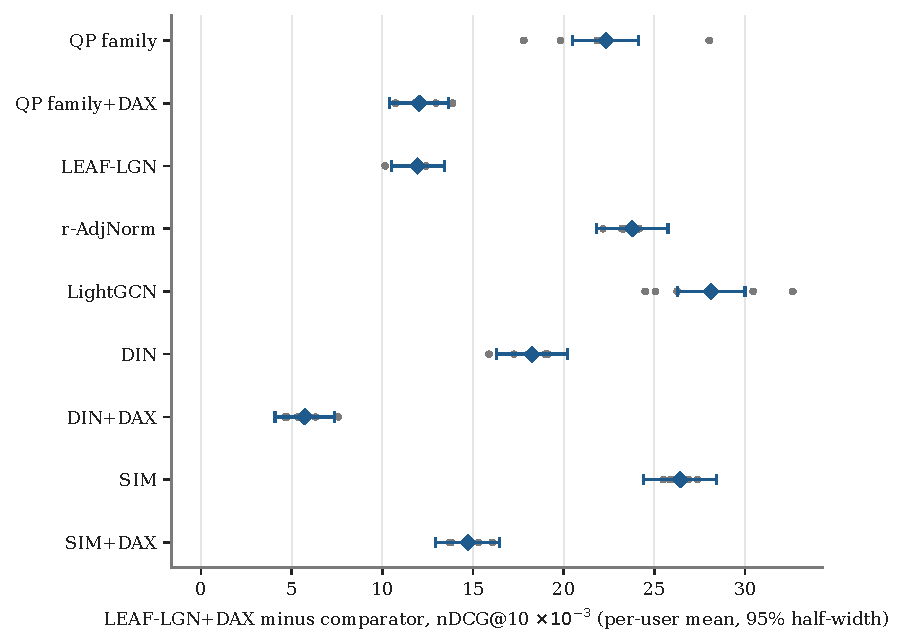
\includegraphics[width=0.85\linewidth]{figs/fig_forest.pdf}
\caption{Paired differences of LEAF-LGN+DAX against each of the thirteen comparators of the main family, in units of $10^{-3}$ nDCG@10.
  Each grey dot is the difference in one of the five splits. The diamond is the pooled per-user mean difference, with its 95\%
  half-width. Positive values favour LEAF-LGN+DAX. SIM denotes SIM-hard, and PW-LightGCN is the propensity-weighted LightGCN.}
\label{fig:forest}
\end{figure}

\subsection{Comparison with the same DAX module}
\label{sec:res-fair}

We ask whether the advantage comes from the DAX module or from the search budget. The answer is that the module accounts for part of it: against PW-LightGCN with the same module (Table~\ref{tab:fair}), LEAF-LGN+DAX is higher by $+12.04$ [1.63], with an adjusted split-level value of 0.0223. PW-LightGCN gains $+10.28$ [1.37]
from DAX on its own backbone, but the split-level p value is 0.105, so that increment is not established at split level. The LEAF-LGN backbone with its
separate search is $+9.63$ [1.60] above PW-LightGCN, with an unadjusted split-level p value of 0.063. The LEAF backbone alone is therefore not established
as an improvement over PW-LightGCN at split level, whereas the combination is. PW-LightGCN with DAX searches only the backbones selected without DAX,
which is conservative for the method.

\begin{table}[tbp]
\centering
\footnotesize
\caption{Fair-baseline reading: the DAX increments, and LEAF-LGN without DAX against the PW-LightGCN, with the configurations searched by each method (first and second method in the second column).}
\label{tab:fair}
\begin{adjustbox}{max width=\linewidth}
\begin{tabular}{lcccc}
\toprule
Comparison & Configurations & Diff.\ [95\% hw] & NB $p$ & NB $p_{\mathrm{Holm}}$ \\
\midrule
LEAF-LGN+DAX minus PW-LightGCN+DAX (fair baseline) & 3,840 / 3,200 & +12.04 [1.63] & 0.006 & $2.23\times10^{-2}$ \\
PW-LightGCN+DAX minus PW-LightGCN (DAX on the PW-LightGCN backbone) & 3,200 / 20 & +10.28 [1.37] & 0.105 & n/a \\
LEAF-LGN+DAX minus LEAF-LGN (DAX on the LEAF backbone) & 3,840 / 12 & +11.96 [1.47] & 0.001 & $8.22\times10^{-3}$ \\
LEAF-LGN (separate search) minus PW-LightGCN & 197 / 20 & +9.63 [1.60] & 0.063 & n/a \\
\bottomrule
\end{tabular}
\end{adjustbox}
\par\smallskip
\begin{minipage}{\linewidth}\raggedright\footnotesize Diff. and NB $p$ are defined as in Table~\ref{tab:main}. NB $p_{\mathrm{Holm}}$ is given for the two comparisons of the main family; the other two values are not adjusted. The PW-LightGCN with DAX searches only the PW-LightGCN backbone configurations selected without DAX.\end{minipage}
\end{table}


\subsection{DAX on six backbones}
\label{sec:res-backbone}

We ask whether DAX helps backbones other than LEAF-LGN. Table~\ref{tab:backbone} gives the six increments. The answer is that the per-user increment is positive on all six, and that the split-level
increment is significant on five after Holm correction over the six. PW-LightGCN is the exception, with a split-level p value of 0.105. The LightGCN
increment depends on its base. Against the LightGCN of the same run it is $+11.60$ [1.51] (adjusted 0.005). Against the four-configuration LightGCN of the
main table it is $+13.73$ [1.46], with an unadjusted split-level p value of 0.091, which is not significant after adjustment over the six (0.182). Each
row uses its own base, so the increments are not comparable with the main difference of LEAF-LGN+DAX.

\begin{table}[tbp]
\centering
\footnotesize
\caption{DAX on six backbones on KuaiRand-27K: nDCG@10 without and with the DAX module, the paired per-user difference in units of $10^{-3}$ with its 95\% half-width, and the split-level Nadeau-Bengio test. SIM denotes SIM-hard.}
\label{tab:backbone}
\begin{adjustbox}{max width=\linewidth}
\begin{tabular}{lrrcc}
\toprule
Backbone & Without DAX & With DAX & Diff.\ [95\% hw] & NB $p$ \\
\midrule
EASE & 0.4507 & 0.4623 & +11.98 [1.64] & 0.000 \\
LightGCN (re-trained) & 0.4597 & 0.4709 & +11.60 [1.51] & 0.001 \\
QP family & 0.4634 & 0.4733 & +10.28 [1.37] & 0.105 \\
LEAF-LGN & 0.4736 & 0.4854 & +11.96 [1.47] & 0.001 \\
DIN & 0.4675 & 0.4796 & +12.53 [1.41] & 0.011 \\
SIM & 0.4590 & 0.4706 & +11.72 [1.46] & 0.008 \\
\bottomrule
\end{tabular}
\end{adjustbox}
\par\smallskip
\begin{minipage}{\linewidth}\raggedright\footnotesize NB $p$ values are not adjusted (no family). LightGCN: the base and the DAX variant come from the same experiment (3 base configurations; 960 with DAX). Against the four-configuration LightGCN of Table~\ref{tab:main} the increment is +13.73 [1.46] (NB $p$ 0.091).\end{minipage}
\end{table}


\subsection{Ablations of DAX}
\label{sec:res-ablate}

We ask which parts of DAX matter. The answer is that the full DAX gain over its base is significant (adjusted 0.037), that permuting attractiveness across items reduces it to zero per user, and that permuting within tags keeps 41.6\% of it. Across items the gain is $-0.27$ [0.36], which is not distinguishable from zero (adjusted
0.754). Within tags it is $+6.28$ [1.10] (adjusted 0.007). Over the three permutation seeds the across-item gains lie between $-0.44$ and $-0.16$, and the
within-tag gains between $+5.66$ and $+6.84$ (Table~\ref{tab:ablate}, lower block). Each removal of a DAX component lowers the per-user score. Removing the scenario factors lowers the score by $1.51$ [0.79], removing the lifelong prior by $1.78$ [0.61], removing the tag prior by $3.41$ [0.99], and the additive model by $6.09$ [0.96]. None of these six full-minus-variant differences is significant at split level: the smallest adjusted value over the six is 0.088.
The per-user evidence therefore favours full DAX over each variant, but the split-level evidence does not separate the three switches or the additive
model from full DAX.

\begin{table}[tbp]
\centering
\footnotesize
\caption{DAX ablations on KuaiRand-27K: gain over the LEAF-LGN base of the ablation experiment, the difference to full DAX, and the permutation controls.}
\label{tab:ablate}
\begin{adjustbox}{max width=\linewidth}
\begin{tabular}{lrcccccc}
\toprule
Variant & Configs & Mean & Gain [95\% hw] & $p_{\mathrm{Holm}}$ & Kept (\%) & Full minus variant & $p_{\mathrm{Holm}}$ \\
\midrule
full DAX & 320 & 0.4854 & +15.10 [1.42] & $8.82\times10^{-95}$ & 100.0 & n/a & n/a \\
without scenario factors $\kappa_t$ & 160 & 0.4839 & +13.59 [1.43] & $1.28\times10^{-76}$ & 90.0 & +1.51 [0.79] & $2.02\times10^{-4}$ \\
without lifelong prior on $\theta_u$ & 160 & 0.4836 & +13.31 [1.43] & $7.92\times10^{-73}$ & 88.2 & +1.78 [0.61] & $2.16\times10^{-8}$ \\
without tag prior on $\alpha_i$ & 160 & 0.4820 & +11.68 [1.22] & $1.28\times10^{-76}$ & 77.4 & +3.41 [0.99] & $4.79\times10^{-11}$ \\
additive logit model with user and scenario effects & 320 & 0.4794 & +9.01 [1.25] & $9.20\times10^{-45}$ & 59.7 & +6.09 [0.96] & $5.43\times10^{-35}$ \\
$\alpha$ permuted across items & 960 & 0.4704 & -0.27 [0.36] & $1.48\times10^{-1}$ & -1.8 & +15.36 [1.40] & $3.53\times10^{-101}$ \\
$\alpha$ permuted within tags & 960 & 0.4768 & +6.28 [1.10] & $1.23\times10^{-28}$ & 41.6 & +8.81 [1.00] & $2.47\times10^{-65}$ \\
\midrule
\multicolumn{8}{l}{Separate permutation seeds (the variants above select over the three seeds)} \\
$\alpha$ permuted across items, seed 0 &  &  & -0.44 [0.50] & NB 0.510 & -2.9 &  &  \\
$\alpha$ permuted across items, seed 1 &  &  & -0.16 [0.53] & NB 0.986 & -1.0 &  &  \\
$\alpha$ permuted across items, seed 2 &  &  & -0.20 [0.51] & NB 0.775 & -1.3 &  &  \\
$\alpha$ permuted within tags, seed 0 &  &  & +5.66 [1.14] & NB 0.010 & 37.5 &  &  \\
$\alpha$ permuted within tags, seed 1 &  &  & +6.84 [1.13] & NB 0.002 & 45.3 &  &  \\
$\alpha$ permuted within tags, seed 2 &  &  & +6.35 [1.24] & NB 0.001 & 42.1 &  &  \\
\bottomrule
\end{tabular}
\end{adjustbox}
\par\smallskip
\begin{minipage}{\linewidth}\raggedright\footnotesize Gain: variant minus the LEAF-LGN base of the ablation experiment (mean 0.4706, two backbone trainings, five values of $\gamma$, epoch window of three around the selection of the main experiment). This base is lower than the LEAF-LGN of Table~\ref{tab:main} (0.4736), so the full gain here (+15.10) exceeds the main increment by 3.14; the variants are compared through the full-minus-variant columns, which do not use the base. Holm: the p values of the gains are adjusted within the seven gains, and those of full minus variant within the six ablated variants. Kept: the gain as a percentage of the full gain of this experiment, so the percentages inherit the base and are approximate. Permutation seeds are separate runs, one per seed.\end{minipage}
\end{table}


The examination structure is tested against a shrunk click rate in Section~\ref{sec:res-exam}.

\subsection{Examination control and stand-alone item scores}
\label{sec:res-exam}

We ask whether the examination model contributes to DAX, and what the item score does without the rest of the model. The answer is that
the examination model contributes, and that the item score is useful only once click rates are corrected for examination. Used alone, DAX
does no better than popularity, so its value lies in complementing a personalised backbone.

The control sets the user and scenario examination factors to one, so that the item score becomes the tag-shrunk click rate of the pre-cut
log, with the same prior strengths, post-hoc combination and validation selection (Table~\ref{tab:exam}). Its search has 80 configurations
against 320, because the examination settings collapse. Setting the factors to one lowers the score by $8.80$ [1.10] against full DAX (NB
$p$ 0.008, adjusted 0.025). The control is still $6.30$ [0.95] above LEAF-LGN trained on the same runs (adjusted 0.045, significant but
narrow). The adjusted values are Holm corrections over the four difference rows of the table.

As stand-alone item scores on the same candidate lists, DAX reaches 0.4206, the tag-shrunk click rate 0.3720 and popularity, the pre-cut click
count, 0.4194, and a random order 0.3307. DAX alone is $+48.56$ [2.48] above the click rate (NB $p$ below 0.001). Against popularity the difference is $+1.40$ [2.84],
which is not significant (NB $p$ 0.620).

\begin{table}[tbp]
\centering
\footnotesize
\caption{Examination control and stand-alone item scores on KuaiRand-27K.}
\label{tab:exam}
\begin{adjustbox}{max width=\linewidth}
\begin{tabular}{lrrrcc}
\toprule
Setting or comparison & Configs & Mean & Difference [95\% hw] & NB $p$ & NB $p_{\mathrm{Holm}}$ \\
\midrule
LEAF-LGN+DAX, examination on & 320 & 0.4854 &  &  &  \\
LEAF-LGN+DAX, examination off & 80 & 0.4767 &  &  &  \\
LEAF-LGN, same trainings & 2 & 0.4706 &  &  &  \\
\midrule
Examination on minus off &  &  & +8.80 [1.10] & 0.008 & 0.025 \\
Examination off minus LEAF-LGN &  &  & +6.30 [0.95] & 0.023 & 0.045 \\
\midrule
Random order (reference, no model) &  & 0.3307 &  &  &  \\
DAX alone & 320 & 0.4206 &  &  &  \\
Tag-shrunk click rate alone (examination off) & 80 & 0.3720 &  &  &  \\
Popularity (pre-cut click count) & 1 & 0.4194 &  &  &  \\
\midrule
DAX alone minus tag-shrunk click rate &  &  & +48.56 [2.48] & $<0.001$ & $<0.001$ \\
DAX alone minus popularity &  &  & +1.40 [2.84] & 0.620 & 0.620 \\
\bottomrule
\end{tabular}
\end{adjustbox}
\par\smallskip
\begin{minipage}{\linewidth}\raggedright\footnotesize Examination on is the full DAX of the ablation search, which reproduces the main test values. Examination off sets the user and scenario examination factors to one, so the item score is the tag-shrunk click rate of the pre-cut log. Both settings use the same prior strengths, the same post-hoc combination and the same validation selection; the examination-off search has fewer configurations because the examination settings collapse. The bottom block scores the same candidate lists with the item score alone, and the random-order row ranks each list at random. Mean: mean of the five split means. Difference: mean over the pooled test users of the paired per-user difference, times $10^{3}$, with the 95\% half-width. NB $p$ is the split-level Nadeau-Bengio value; NB $p_{\mathrm{Holm}}$ is Holm correction over the four difference rows.\end{minipage}
\end{table}


Two simpler item scores serve as controls: log popularity, the logarithm of one plus the pre-cut clicks of an item, and the raw
pre-cut click rate. Added to LEAF-LGN in the same post-hoc combination, with the same trainings, weights and validation selection,
log popularity gives 0.4711 and the raw click rate 0.4744, against 0.4706 for LEAF-LGN alone and 0.4854 for LEAF-LGN+DAX in the same
setting (Table~\ref{tab:item}). The gain of DAX over these two item scores is $+14.68$ [1.37] and $+11.27$ [1.26] per user, with
split-level p values 0.005 and 0.002 (adjusted 0.011 and 0.005 over the three difference rows of the table). The gain therefore does
not come from popularity or from click rate alone. The user-group refinement is optional: without it, DAX scores 0.4844, a difference
of $+1.13$ [0.53] with split-level p 0.377, which is no detectable contribution.

\begin{table}[tbp]
\centering
\footnotesize
\caption{Item-term controls on KuaiRand-27K: LEAF-LGN with log popularity or the raw click rate of each item in place of DAX, and DAX without user groups (nDCG@10).}
\label{tab:item}
\begin{adjustbox}{max width=\linewidth}
\begin{tabular}{lrrrcc}
\toprule
Setting or comparison & Configs & Mean & Difference [95\% hw] & NB $p$ & NB $p_{\mathrm{Holm}}$ \\
\midrule
LEAF-LGN, same trainings & 2 & 0.4706 &  &  &  \\
LEAF-LGN + log popularity & 10 & 0.4711 &  &  &  \\
LEAF-LGN + raw pre-cut click rate & 10 & 0.4744 &  &  &  \\
\midrule
LEAF-LGN+DAX & 320 & 0.4854 &  &  &  \\
LEAF-LGN+DAX without user groups & 160 & 0.4844 &  &  &  \\
\midrule
LEAF-LGN+DAX minus LEAF-LGN + log popularity &  &  & +14.68 [1.37] & 0.005 & 0.011 \\
LEAF-LGN+DAX minus LEAF-LGN + raw click rate &  &  & +11.27 [1.26] & 0.002 & 0.005 \\
LEAF-LGN+DAX minus LEAF-LGN+DAX without user groups &  &  & +1.13 [0.53] & 0.377 & 0.377 \\
\bottomrule
\end{tabular}
\end{adjustbox}
\par\smallskip
\begin{minipage}{\linewidth}\raggedright\footnotesize Log popularity is $\log(1+x)$, where $x$ is the number of clicks on the item before the cut-off. The raw click rate is $(x+1)/(n+2)$, where $n$ is the number of pre-cut impressions of the item. Each item term enters the same post-hoc combination as DAX, with the same trainings, the same weight grid and the same validation selection. The last row removes the user-group refinement of DAX and keeps everything else. Mean: mean of the five split means. Difference: mean over the pooled test users of the paired per-user difference, times $10^{3}$, with the 95\% half-width. NB $p$ is the split-level Nadeau-Bengio value; NB $p_{\mathrm{Holm}}$ is Holm correction over the three difference rows.\end{minipage}
\end{table}


\subsection{Lifelong deep baselines}
\label{sec:res-deep}

We ask whether lifelong deep models do as well. The answer is no on the main family. DIN is $+18.26$ [1.97] below LEAF-LGN+DAX (adjusted 0.0077) and SIM-hard is
$+26.44$ [2.01] below it (adjusted 0.0003). With DAX, DIN+DAX (0.4796) is $+5.73$ [1.64] below (adjusted 0.0456, significant but narrow), and SIM+DAX (0.4706)
is $+14.72$ [1.77] below (adjusted 0.0061). On KuaiRand-1K the same order holds. Those differences are not adjusted and are not called significant
(Table~\ref{tab:deep}). Each default deep baseline is tuned over four configurations, so the deep models are tuned less widely than LEAF-LGN.

With matched capacity the deep models still fall short. We ran DIN and SIM-hard with embedding and hidden dimension 64, at most 20 epochs
with patience 2, a learning rate of $10^{-2}$ and two weight decays, with and without DAX. DIN reaches 0.4624 and SIM-hard 0.4573, and their
+DAX variants reach 0.4759 and 0.4688. LEAF-LGN+DAX is $+23.35$ [1.97] above DIN, $+9.67$ [1.83] above DIN+DAX, $+28.17$ [2.24] above SIM-hard
and $+16.86$ [1.88] above SIM+DAX. The split-level p values in Table~\ref{tab:deep} are unadjusted, and Holm correction over these four
comparisons keeps every one below 0.05. The larger dimension did not help the deep models in these runs (DIN falls from 0.4675 to 0.4624, and DIN+DAX from 0.4796 to 0.4759), so capacity alone does not close the gap, although these runs are less tuned (Section~\ref{sec:limits}).

\begin{table}[tbp]
\centering
\footnotesize
\caption{Lifelong deep baselines (DIN and SIM-hard) with and without DAX, and their paired difference to LEAF-LGN+DAX (LEAF-LGN+DAX minus the comparator, x1e-3 nDCG@10).}
\label{tab:deep}
\begin{adjustbox}{max width=\linewidth}
\begin{tabular}{lrccccc}
\toprule
Comparator & Mean & Configs & Diff.\ [95\% hw] & $p$ & NB $p$ \\
\midrule
\multicolumn{6}{l}{KuaiRand-27K} \\
DIN & 0.4675 & 4 & +18.26 [1.97] & $1.41\times10^{-73}$ & 0.001 \\
DIN+DAX & 0.4796 & 1280 & +5.73 [1.64] & $7.95\times10^{-12}$ & 0.043 \\
SIM & 0.4590 & 4 & +26.44 [2.01] & $3.55\times10^{-144}$ & 0.000 \\
SIM+DAX & 0.4706 & 1280 & +14.72 [1.77] & $1.39\times10^{-59}$ & 0.001 \\
\midrule
\multicolumn{6}{l}{KuaiRand-1K} \\
DIN & 0.4189 & 4 & +39.26 [10.37] & $2.63\times10^{-13}$ & 0.002 \\
DIN+DAX & 0.4228 & 1280 & +35.89 [9.25] & $7.10\times10^{-14}$ & 0.002 \\
SIM & 0.4246 & 4 & +35.26 [9.24] & $1.70\times10^{-13}$ & 0.007 \\
SIM+DAX & 0.4357 & 1280 & +23.29 [8.69] & $1.81\times10^{-7}$ & 0.095 \\
\midrule
\multicolumn{6}{l}{Lifelong sequence models: DIN attends over the last 200 lifelong events; SIM-hard keeps the 50 most recent events sharing the candidate's tag or author.} \\
\bottomrule
\end{tabular}
\end{adjustbox}
\par\smallskip
\begin{minipage}{\linewidth}\raggedright\footnotesize Raw p values. DIN and SIM are tuned over four configurations (lr {1e-2, 3e-3} times wd {1e-4, 1e-5}) with patience 2; their +DAX arms use the post-hoc DAX grid. Entries marked TBD have no result file yet.\end{minipage}
\end{table}


\subsection{Controls}
\label{sec:res-controls}

We ask whether the signals depend on what they are meant to capture. The lifelong channels do. Removing them from LEAF-LGN lowers the score by $11.46$ [1.71] (Table~\ref{tab:leafctl-lgn})
(adjusted 0.036 over the three controls). Shuffling the users' lifelong tables across users lowers it by $10.65$ [1.77] (adjusted 0.005), to a level
close to the model without lifelong channels. The gain therefore depends on each user's own history rather than on lifelong features in general.
Removing the policy channel does not lower the score. The variant without it scores $0.55$ [0.33] higher (adjusted 0.793) and gives identical test scores in four of the five splits. These controls use the separately tuned LEAF-LGN, not LEAF-LGN+DAX. The controls on a closed-form scorer in \ref{app:leafctl} agree
in direction.

\begin{table}[tbp]
\centering
\footnotesize
\caption{LEAF-LGN controls on KuaiRand-27K: the reference against the same model with the lifelong channels removed, with the lifelong tables shuffled across users, and with the policy channel removed (nDCG@10).}
\label{tab:leafctl-lgn}
\begin{adjustbox}{max width=\linewidth}
\begin{tabular}{lrrrrr}
\toprule
Variant & Configurations & Mean & Difference [95\% hw] & Per-user $p$ & NB $p$ \\
\midrule
LEAF-LGN (independent tuning, reference) & 197 & 0.4728 & n/a & n/a & n/a \\
\midrule
without lifelong channels & 12 & 0.4614 & +11.46 [1.71] & $2.82\times10^{-39}$ & 0.018 \\
lifelong tables shuffled across users & 12 & 0.4624 & +10.65 [1.77] & $4.04\times10^{-32}$ & 0.002 \\
without policy channel & 4 & 0.4733 & -0.55 [0.33] & $1.13\times10^{-3}$ & 0.793 \\
\bottomrule
\end{tabular}
\end{adjustbox}
\par\smallskip
\begin{minipage}{\linewidth}\raggedright\footnotesize Difference: the reference minus the variant, so a positive value means the removed signal helps. Each variant is selected on validation users over its own grid (12, 12, 4 configurations), and the reference over 197 configurations, which favours the reference. Per-user $p$: two-sided paired t test over the pooled test users. NB $p$: Nadeau-Bengio test over the five split means. Neither is adjusted for the three variants.\end{minipage}
\end{table}


\subsection{KuaiRand-1K replication}
\label{sec:res-1k}

We ask whether the result holds on the smaller release. The answer is yes in direction and size, with wider intervals. On 842 pooled test users,
LEAF-LGN+DAX (0.4590) is $+37.58$ [11.10] above PW-LightGCN (0.4246, adjusted 0.0228) and $+25.82$ [9.66] above PW-LightGCN with DAX (0.4358, adjusted
0.0218). The DAX increment on PW-LightGCN, $+11.76$ [8.54], is not significant (adjusted 0.160). The table is in \ref{app:counts}.

\subsection{Training seeds}
\label{sec:res-seeds}

We ask whether the result is specific to one training seed. The gain is positive in every seed tested, and the two narrow comparisons keep their margins under the same seeds, but the evidence is limited. The LEAF-LGN+DAX mean is
0.4854 for seed 0, and 0.4858, 0.4856 and 0.4844 for seeds 1 to 3, a spread of $0.4853\pm0.0006$. Seeds 1 to 3 use a reduced backbone search, and their
bases are lower (0.4714, 0.4708 and 0.4716), so their gains of $+14.67$, $+15.10$ and $+12.89$ are not comparable with the seed-0 gain of $+11.96$ [1.47].
Their split-level p values are unadjusted, between 0.0009 and 0.0023. Table~\ref{tab:seeds} in \ref{app:supp} gives the seeds.

The closest comparator was also re-trained under seeds 1 and 2, with its default configuration grid, and compared with LEAF-LGN+DAX under
the same seed (Table~\ref{tab:seeds-din}). LEAF-LGN+DAX, with its reduced backbone search of Table~\ref{tab:seeds}, is higher in both: by $+9.99$ [1.66] under seed 1 (0.4858 against 0.4756, NB $p$
0.011) and by $+6.76$ [1.79] under seed 2 (0.4856 against 0.4785, NB $p$ 0.004). Both split-level values are below 0.05 unadjusted and after
Holm correction over the two seeds, so the margin over DIN with DAX is not specific to seed 0. 

\begin{table}[tbp]
\centering
\footnotesize
\caption{Training seeds 1 and 2 on KuaiRand-27K: LEAF-LGN+DAX against DIN+DAX, each re-trained with the same seed.}
\label{tab:seeds-din}
\begin{adjustbox}{max width=\linewidth}
\begin{tabular}{lrrrcc}
\toprule
Seed & LEAF-LGN+DAX & DIN+DAX & Difference [95\% hw] & NB $p$ & NB $p_{\mathrm{Holm}}$ \\
\midrule
1 & 0.4858 & 0.4756 & +9.99 [1.66] & 0.011 & 0.011 \\
2 & 0.4856 & 0.4785 & +6.76 [1.79] & 0.004 & 0.009 \\
\bottomrule
\end{tabular}
\end{adjustbox}
\par\smallskip
\begin{minipage}{\linewidth}\raggedright\footnotesize Difference: LEAF-LGN+DAX minus DIN+DAX, in units of $10^{-3}$ nDCG@10 per user, with the 95\% half-width. The LEAF-LGN+DAX values are those of Table~\ref{tab:seeds}; DIN+DAX is searched over its default configuration grid in each seed. NB $p$ is split-level. Holm correction runs over the two seeds.\end{minipage}
\end{table}


The PW-LightGCN comparator and its DAX variant were also re-trained under seeds 1 and 2, at the configurations chosen in the main comparison, with the epoch within three of the chosen epoch and the DAX grid and mixing weights of the main comparison (Table~\ref{tab:seeds-pw}). LEAF-LGN+DAX is higher in both seeds: by $+22.60$ [1.90] under seed 1 (0.4858 against 0.4635) and by $+21.84$ [1.93] under seed 2 (0.4856 against 0.4639). The margin is therefore unchanged from the main comparison, at about $22\times10^{-3}$, and the split-level p values are below 0.001 under both seeds after Holm correction over the two seeds. The margin of LEAF-LGN+DAX over the DAX variant of PW-LightGCN is $+13.76$ [1.62] under seed 1 (0.4858 against 0.4721) and $+13.32$ [1.62] under seed 2 (0.4856 against 0.4722), with Holm-adjusted split-level values of 0.004 and 0.001. The other comparators remain single-seed: DIN, SIM, SIM+DAX, r-AdjNorm, LightGCN, EASE, the DAX variants of LightGCN and EASE, and the four published estimators.

\begin{table}[tbp]
\centering
\footnotesize
\caption{Training seeds 1 and 2 on KuaiRand-27K: LEAF-LGN+DAX against PW-LightGCN and PW-LightGCN+DAX, each re-trained with the same seed.}
\label{tab:seeds-pw}
\begin{adjustbox}{max width=\linewidth}
\begin{tabular}{llrrrcc}
\toprule
Seed & Comparator & LEAF-LGN+DAX & Comparator mean & Difference [95\% hw] & NB $p$ & NB $p_{\mathrm{Holm}}$ \\
\midrule
1 & PW-LightGCN & 0.4858 & 0.4635 & +22.60 [1.90] & $<0.001$ & $<0.001$ \\
1 & PW-LightGCN+DAX & 0.4858 & 0.4721 & +13.76 [1.62] & 0.004 & 0.004 \\
2 & PW-LightGCN & 0.4856 & 0.4639 & +21.84 [1.93] & $<0.001$ & $<0.001$ \\
2 & PW-LightGCN+DAX & 0.4856 & 0.4722 & +13.32 [1.62] & $<0.001$ & 0.001 \\
\bottomrule
\end{tabular}
\end{adjustbox}
\par\smallskip
\begin{minipage}{\linewidth}\raggedright\footnotesize Difference: LEAF-LGN+DAX minus the comparator, in units of $10^{-3}$ nDCG@10 per user, with the 95\% half-width. The LEAF-LGN+DAX values are those of Table~\ref{tab:seeds}. Each comparator is re-trained with the configurations chosen in the main run, with the epoch within three of the chosen epoch and the DAX grid and mixing weights as in the main run. NB $p$ is split-level. Holm correction runs over the two seeds of each comparator.\end{minipage}
\end{table}


\section{Discussion}\label{sec:discussion}

\paragraph{Why the multiplicative form} The additive alternative keeps the same covariates and scenario effects, but replaces
the product of user examination and item attractiveness by an additive logit. Its loss against full DAX is the largest of the
structural comparisons in Section~\ref{sec:res-ablate}. The difference is easiest to see for the cooking clip. Under the
multiplicative model, a non-click from a viewer who rarely examines videos, or in a scenario where few videos are examined,
barely lowers the estimated attractiveness of the clip, because such a non-click is weak evidence against the clip. Under the
additive model, once the user effect is absorbed, the same non-click lowers the item effect as much as any other non-click,
and the two cases are treated alike. This is a fit comparison under one protocol. It does not show that the multiplicative form
is correct in an absolute sense.

\paragraph{Item-level and tag-level parts} Permuting attractiveness within tags keeps part of the gain, and permuting it across
items removes all of it. A tag mean alone would therefore capture part of the signal, and the remainder is carried by item
deviations from that mean. The permutations keep the marginal distribution of $\alpha$ fixed, so the decomposition is only as
strong as these controls.

\paragraph{Lifelong channels} On LEAF-LGN, shuffling the lifelong tables across users removes the lifelong gain, and removing the
policy channel does not lower the score, so the policy channel brings no measurable gain (Section~\ref{sec:res-controls}). The
closed-form variant shows a small per-user contribution from the policy channel that is not significant at the split level
(\ref{app:leafctl}). The signal that transfers to randomly exposed items is therefore mainly the users' own lifelong affinities
for content keys.

\paragraph{Complementarity} DAX is used as an increment on top of a backbone, and the tables report only that increment. Under
the combination rule of Section~\ref{sec:method-combine}, its score carries information that the backbone scores do not. DAX is
not reported as a stand-alone ranker.

\paragraph{Published debiased estimators} NAVIP is close to LightGCN, and the three matrix factorisation estimators are far below the
tuned baselines. Each was tuned over four configurations, so whether a wider search would change their ordering is open, as it is
for the deep baselines.

\paragraph{Lifelong deep models} DIN+DAX is the closest comparator of the main family, and LEAF-LGN+DAX is above it with a
borderline split-level value (Section~\ref{sec:res-deep}). The deep baselines are tuned over four configurations each, so whether
a wider search would change the ordering is open.

\paragraph{Remaining headroom} The gains come from the item-level appeal estimate and from the lifelong user channels. Further
gains would need a different source of information about item quality for random viewers, such as richer content or a direct
measurement of responses to uniform exposure, and not a larger search over the present hyperparameters. This is an interpretation
of the controls and not a tested claim.

\section{Limitations}
\label{sec:limits}

The paper does not claim unbiasedness, causal identification of item quality, or generality beyond one platform family. The limitations
below set the scope of the results.

\paragraph{One platform family} KuaiRand-27K and KuaiRand-1K come from one platform and one period, with overlapping users. The 1K users are a
subset of the 27K users, so the 1K results are not an independent replication.

\paragraph{Few splits and low power} The main comparisons use five user-level splits, and the split-level test has low power. Two adjusted values
are 0.0456, so the two narrow comparisons would need more splits to be firmly established. The per-user test gives far smaller values, but it treats users
as independent across splits, which they are not.

\paragraph{Examination and user taste} The examination control sets the examination factors to one in a single setting, on one platform,
and its comparison is one of four in its family. Examination and user taste are also confounded by construction, because the centre of
the examination prior is the user's lifelong click rate. The attractiveness is therefore a model-based quantity under strong assumptions,
and part of the gain may reflect user activity rather than examination.

\paragraph{The combination is fitted after training} The mixing weight $\gamma$ is selected on validation users, and DAX is not trained jointly with
the backbone in the reported results. We did not evaluate a variant in which $\gamma$ is learned jointly with the backbone.

\paragraph{Unequal budgets and grid edges} LEAF-LGN+DAX searches 3,840 configurations per split, PW-LightGCN 20, and PW-LightGCN with DAX 3,200. On
KuaiRand-1K, PW-LightGCN with DAX searches 6,400 configurations, which favours the baseline. The prior strength $\nu$ and the lifelong strength
$\lambda$ were selected at the edges of the default grid. A wider grid, with $\nu$ in $\{10,20,40,80,160\}$ and $\lambda$ in $\{0,100,200,400,1000\}$,
gives 0.4860 against 0.4854, a difference of $+0.55$ [0.52] (split-level Nadeau-Bengio p 0.367, unadjusted). The default grid therefore does not
limit the test score, although the selected prior strength depends on the grid (\ref{app:grids}).

\paragraph{Identifiability up to scale} The examination and attractiveness factors are identified only up to a scale shared by $\theta_u$ and
$\alpha_i$. The order of $\alpha_i$ is unaffected, but the logit used in the combination is not scale-invariant, so the prior strengths are
validation hyperparameters.

\paragraph{Reduced runs and separate searches} The ablations and the seeds of LEAF-LGN+DAX use reduced grids (Sections~\ref{sec:res-ablate}
and~\ref{sec:res-seeds}), so their gains are not compared with the main increment. Two further seeds were run for DIN+DAX as well, and PW-LightGCN
was not re-trained under other seeds. The LEAF-LGN controls use the separately tuned model, with 12, 12 and 4 configurations against 197 for the
reference, which favours the reference. The closed-form controls were run on the closed-form LEAF scorer, not on a graph model. The headline
LEAF-LGN+DAX backbone selects a policy weight of 0.25 or 0.5, and the DAX increment on LEAF-LGN compares it with a backbone that selects 0.

\paragraph{Deep and published baselines} DIN and SIM-hard are each tuned over four configurations, and the four published estimators over four
configurations each. The matched-capacity runs of the deep models use two configurations for each plain model and 640 for each +DAX variant. A
deeper search, or a sequence length other than 200 for DIN, may close the gap; we did not test either.

\paragraph{Click label only} We used the click label only. We did not evaluate a long-view label, or a protocol in which the training log extends
past $T_0$ for the full model.

\paragraph{Content and scenario} The content keys are the tag, the author and the music track, and the evaluation scenario is the one with
$\kappa_1=1$. The transfer of the scenario factors to other scenarios is not tested, and the combination does not close the item-level gap to the
uniform-rate oracle (Section~\ref{sec:res-headroom}).

\section{Conclusion}\label{sec:conclusion}

When a graph recommender is evaluated on items inserted uniformly at random into feeds, two log-only signals help it rank those
items. Lifelong, exposure-conditional affinities of users for content keys (LEAF) transfer from items outside the test pool through
content keys, and the gain disappears when the users' lifelong tables are shuffled. A detection-adjusted item attractiveness (DAX),
fitted by EM to a click model that discounts non-clicks by user and scenario examination, adds an increment on top of six backbones.
The increment vanishes when attractiveness is shuffled across items, and within-tag shuffles keep part of it.

On KuaiRand-27K, under a temporal protocol with five user-level splits, LEAF-LGN with DAX is higher than each of the nine comparators
of the main family. The per-user Holm-adjusted p values are below $10^{-11}$, and the split-level Holm-adjusted values are at most
$4.56\times10^{-2}$, which is borderline for the QP family and for DIN with DAX. Against the QP family with DAX, the fair baseline,
the difference is $+12.04$ [1.63]. On KuaiRand-1K the gain over the QP family holds. The within-seed gain over LEAF-LGN is positive
for training seeds 1 to 3, on a reduced grid.

The evidence comes from one platform family, five splits and search budgets that differ by two orders of magnitude. The results are
a controlled ranking gain under the stated protocol and an increment of the module on six backbones.

\section*{Data and code availability}
The KuaiRand data are publicly available \citep{gao2022kuairand}. The code will be made available upon publication.
\bibliographystyle{elsarticle-harv}
\bibliography{../refs,refs_new}
\appendix
\section{The QP family}\label{app:qp}

The QP family is our own baseline. It has not been published, and it is described here in full so that the
baseline can be reproduced. It is a weighted Bayesian personalised ranking (BPR) objective
\citep{rendle2009bpr} on a LightGCN backbone, with three variants, DR-BPR-LGN-1, DR-BPR-LGN-p2 and DR-BPR-LGN-p. The variants
differ only in an offset term, and each is trained on the same pre-cut in-pool log as LEAF-LGN.

\paragraph{Exposure model} The probability $P_{ui}$ that item $i$ was exposed to user $u$ comes from a logistic exposure model,
$P_{ui}=\sigma\bigl(a+b\,\operatorname{logit}r_u+c\,\operatorname{logit}r_i\bigr)$, where $r_u$ and $r_i$ are the exposure rates of
the user and of the item in the policy log. The coefficients are fitted by maximum likelihood on the policy log, and a feature with no
variation is dropped. The propensities are clipped below at 0.05.

\paragraph{Imputation} The outcome imputation $\hat Y_{ui}$ is an additive model of user and item effects fitted with
inverse-propensity weights, clipped to $[0,1]$ for the weights and to $[0.01, 0.99]$ for the offset. Its standardised logit $z_{ui}$
is the offset feature.

\paragraph{Unlogged-pair weight} For a pair that is not a logged positive, $Q_{ui}=\hat Y_{ui}(1-P_{ui})/(1-P_{ui}\hat Y_{ui})$,
clipped to $[0,1]$. It is the probability that such a pair is a positive after all, under $Y$ independent of exposure given the
imputation.

\paragraph{Loss} For a logged positive pair $(u,i)$ and a sampled negative $j$ (resampled when $(u,j)$ is a logged positive), the
weight of the negative is $w_{uj}=\max(1-Q_{uj},10^{-3})$ and the loss is
\[
\mathcal L=-\frac{\sum_{(u,i,j)} w_{uj}\log\sigma(s_{ui}-s_{uj})}{\sum_{(u,i,j)} w_{uj}},
\]
with the score $s_{ui}=\langle e_u,e_i\rangle+\beta\,z_{ui}$. The DR-BPR-LGN-1 variant has $\beta=0$. The DR-BPR-LGN-p2 and
DR-BPR-LGN-p variants use $\beta\in\{1,2\}$ and $\beta\in\{0.5,1\}$ respectively.

\paragraph{Grids and selection} The backbone is LightGCN with two layers and dimension 64. The grid is learning rate in
$\{10^{-2}, 3\times10^{-3}\}$ and weight decay in $\{10^{-5}, 10^{-4}\}$, with the offset grid above. That gives 4 configurations
for DR-BPR-LGN-1, 8 for DR-BPR-LGN-p2 and 8 for DR-BPR-LGN-p, 20 in total. Training runs for at most 40 epochs with patience 3,
and batch size 8,192. Validation nDCG@10 selects the configuration in each split. The QP family in the main comparison is the
variant with the largest validation value in each split, so its search is 20 configurations per split. The QP family with DAX
(Section~\ref{sec:res-fair}) reuses the QP backbones selected without DAX.

\section{EM for detection-adjusted attractiveness}\label{app:em}

This appendix gives the complete model and updates. Only rows with time before the cut-off $T_0$ are read.

\paragraph{Model} A logged impression of user $u$, item $i$ and scenario $t$ has an examination indicator $E$ and an attraction indicator $R$,
\[
E\sim\mathrm{Bernoulli}(\theta_u\kappa_t),\qquad R\sim\mathrm{Bernoulli}(\alpha_i),\qquad y=ER,
\]
where $y$ is the click. The factors are in $[0,1]$, except that the scenario factors are relative to the evaluation scenario, with $\kappa_1=1$.

\paragraph{Priors} The priors are $\alpha_i\sim\mathrm{Beta}\bigl(\nu c_{g(i)},\,\nu(1-c_{g(i)})\bigr)$ with $\nu$ the prior strength (80 or 160 in the search,
80 in the main experiment), $\theta_u\sim\mathrm{Beta}\bigl(\lambda\tilde c_u,\,\lambda(1-\tilde c_u)\bigr)$ with $\lambda$ the lifelong strength (100 in the
main experiment, or 0), and $\kappa_t$ free. The lifelong centre $\tilde c_u$ is the rescaled lifelong rate of Equation~\eqref{eq:life-centre}, clipped
to $[10^{-3},1]$. With $\lambda=0$ we use $\mathrm{Beta}(2,2)$ on $\theta_u$. The tag centre $c_g$ is the pooled attraction of the items of tag $g$ with
a $\mathrm{Beta}(1,1)$ smoothing. In the content-regression variant the centre $c_{g(i)}$ is replaced, after five iterations, by a weighted ridge
regression (penalty 10) of $\operatorname{logit}\alpha$ on one-hot content codes with weights $\sqrt{n_i+1}$.

\paragraph{Initialisation and iterations} $\theta_u=0.7$, $\kappa_t=1$, $\alpha_i=0.6$. There are 40 EM iterations, and no convergence test is applied.

\paragraph{E-step} Let $\tau=\theta_u\kappa_t$. A click gives $P(E=1)=P(R=1)=1$. A non-click gives
\[
P(E=1\mid y=0)=\frac{\tau(1-\alpha_i)}{1-\tau\alpha_i},\qquad
P(R=1\mid y=0)=\frac{(1-\tau)\alpha_i}{1-\tau\alpha_i}.
\]

\paragraph{M-step} Let $S^E_u=\sum P(E=1)$ over the rows of $u$ and $K_u=\sum\kappa_t$ over the same rows. Then
\[
\theta_u=\frac{S^E_u+\lambda\,\tilde c_u}{K_u+\lambda}\quad(\lambda>0),\qquad \theta_u=\frac{S^E_u+1}{K_u+2}\quad(\lambda=0),
\]
clipped to $[10^{-3},1]$. For the scenario factors,
\[
\kappa_t=\frac{\sum_{\text{rows of }t}P(E=1)+1}{\sum_{\text{rows of }t}\theta_{u}+1},
\]
and all $\kappa_t$ are divided by the value of the evaluation scenario after each update, so that it equals one. The attractiveness update is
\[
\alpha_i=\frac{\sum_{\text{rows of }i}P(R=1)+\nu\,c_{g(i)}}{n_i+\nu},
\]
clipped to $[10^{-4},1-10^{-4}]$, where $n_i$ is the number of pre-cut rows of item $i$.

\paragraph{Exactness of the closed-form updates} Let $a_u$ and $b_u$ be the prior pseudo-counts of $\theta_u$, with $a_u=\lambda\tilde c_u$ and
$b_u=\lambda(1-\tilde c_u)$ when $\lambda>0$, and $a_u=b_u=1$ when $\lambda=0$. The $\theta_u$ update above is then
$(S^E_u+a_u)/(K_u+a_u+b_u)$. Its stationarity condition for the expected complete-data log-likelihood is
\[
\sum_{r:\,u_r=u}\Bigl[\frac{P(E_r=1)}{\theta_u}-\frac{\kappa_{t_r}\bigl(1-P(E_r=1)\bigr)}{1-\theta_u\kappa_{t_r}}\Bigr]+\frac{a_u}{\theta_u}-\frac{b_u}{1-\theta_u}=0.
\]
Without the pseudo-counts, this reduces to $\sum_r P(E_r=1)=\theta_u\sum_r\kappa_{t_r}$ when $\kappa_{t_r}$ is the same for every row of $u$, which holds
when all of a user's impressions come from one scenario, and then the ratio form is exact. The $\kappa_t$ update has the same property: without the
pseudo-counts it is exact only when $\theta_{u_r}$ is the same for every row of the scenario $t$. In general both updates are approximations, and
the pseudo-counts move them further from the stationary point. The updates also clamp the values: the E-step product $\tau$ to
$[10^{-6},1-10^{-6}]$, the E-step denominator $1-\tau\alpha_i$ from below at $10^{-9}$, $\theta_u$, $\kappa_t$ and the lifelong centre to
$[10^{-3},1]$, and $\alpha_i$ to $[10^{-4},1-10^{-4}]$.

\paragraph{Check of the closed-form updates} We checked the updates on the full pre-cut data of KuaiRand-27K at the configuration chosen most
often on validation (prior 80, tag centre, lifelong strength 100, scenario factors on), recomputing the examination probabilities at the fitted
values. The median user has 88\% of her pre-cut impressions in one scenario (impression-weighted 80\%, and 25\% of users see one scenario). For
$\theta_u$, the ratio and exact updates differ by a median relative amount of 0.2\% (90th percentile 1.3\%), and their Spearman correlation is
0.998. For $\kappa_t$ they differ by 4.7\% for a non-evaluation scenario with 13\% of the pre-cut impressions, by 18\% for one with 6.6\%, and by up
to 35\% for scenarios with under 0.1\% of the impressions. Fitting the whole model with exact M-steps for $\theta$ and $\kappa$ raises the
observed-data log-likelihood of the pre-cut impressions from $-0.5558$ to $-0.5504$ per impression. The item scores hardly change (Spearman
correlation 0.998 for the logit attractiveness). LEAF-LGN+DAX reaches 0.4859 with exact M-steps against 0.4854 with the ratio updates, a paired
difference of $-0.44$ [0.42] with split-level $p$ 0.153, so the approximation does not change the ranking significantly.

\paragraph{User-group refinement} The attractiveness may also be estimated separately for six groups of users: five quantile groups of the lifelong
base rate $r_u$, and a group without lifelong history. Each group's attractiveness is shrunk towards the overall attractiveness,
\[
\alpha_{i,s}=\frac{\sum_{r:\,i_r=i,\ s(u_r)=s}P(R_r=1)+\nu_{\mathrm g}\,\alpha_i}{n_{is}+\nu_{\mathrm g}},
\]
where $s(u)$ is the group of $u$, $n_{is}$ counts the pre-cut impressions of $i$ to group $s$, and $\nu_{\mathrm g}=80$ is a fixed strength (it is not
tuned). A candidate then uses the attractiveness of its user's group, $\zeta_{ui}=(\operatorname{logit}\alpha_{i,s(u)}-\mu_\alpha)/\sigma_\alpha$, with the same
$\mu_\alpha$ and $\sigma_\alpha$ as in Equation~\eqref{eq:zeta}. The refinement was on in all five splits of the reported model. Without it, DAX
scores 0.4844 against 0.4854 (Section~\ref{sec:res-exam}), so it adds no measurable gain, and it is kept only because it was selected on validation users.

\paragraph{Output} The fit returns $\operatorname{logit}\alpha_i$, $\theta_u$ and $\kappa_t$. The combined score of Section~\ref{sec:method-combine} uses
$\operatorname{logit}\alpha_i$ standardised over the pool, as in Equation~\eqref{eq:zeta}, or the group attractiveness of the user when the
user-group refinement is used.

\section{Grids and chosen configurations}\label{app:grids}

The search spaces are as follows. LEAF-LGN and the other graph backbones use learning rate $\{10^{-2}, 3\times10^{-3}\}$ and
weight decay $\{10^{-4}, 10^{-5}\}$, with the backbone's own grid. LEAF-LGN uses $w\in\{0, 0.25, 0.5\}$ (its policy weight). EASE
uses $w\in\{0,0.25,0.5\}$, $\lambda_{\mathrm{EASE}}\in\{10^{3},3\times10^{3},10^{4}\}$ and a popularity weight
$\beta\in\{0,0.25,0.5\}$, which gives 27 configurations. The DAX grid has 32 configurations: prior strength $\nu\in\{80,160\}$, centre
(tag mean or content regression), lifelong strength $\lambda\in\{0,100\}$, scenario factors on or off, and user groups off or on
with strength 80. The values of $\gamma$ are $\{0, 0.05, 0.1, 0.15, 0.2, 0.3, 0.4, 0.5, 0.7, 1.0\}$. A DAX search multiplies the
backbone trainings by the 32 DAX configurations and the 10 values of $\gamma$, for example $12\times32\times10=3{,}840$ for LEAF-LGN+DAX
and $27\times32\times10=8{,}640$ for EASE+DAX. The QP family with DAX searches 10 backbone trainings, or $10\times32\times10=3{,}200$,
and the search on KuaiRand-1K covers 20 trainings, or 6,400 (\ref{app:qp}).

Table~\ref{tab:extgrid} repeats the comparison with a wider DAX grid: prior strength in $\{10,20,40,80,160\}$ and lifelong strength in
$\{0,100,200,400,1000\}$, under the same reduced set of values of $\gamma$ and the same epoch window as the default grid. The wider grid
gives 0.4860 against 0.4854, a paired per-user difference of $+0.55$ [0.52] ($\times10^{-3}$) with Nadeau-Bengio $p=0.367$. The five
splits choose the pairs (10, 400), (20, 100), (20, 400), (40, 100) and (40, 400) for (prior strength, lifelong strength). The chosen
lifelong strengths lie inside the wider grid, and the chosen prior strengths are below the default values, so the default choice
was not limiting for the test score.

\begin{table}[tbp]
\centering
\footnotesize
\caption{Extended DAX grid on KuaiRand-27K: LEAF-LGN+DAX with prior strength in $\{10,20,40,80,160\}$ and lifelong strength in $\{0,100,200,400,1000\}$, against the default grid (prior $\{80,160\}$, lifelong strength $\{0,100\}$), nDCG@10.}
\label{tab:extgrid}
\begin{adjustbox}{max width=\linewidth}
\begin{tabular}{lrrrr}
\toprule
Grid & Configurations & Mean & Difference from default [95\% hw] & NB $p$ \\
\midrule
Default grid & 320 & 0.4854 & n/a & n/a \\
Extended grid & 2,000 & 0.4860 & +0.55 [0.52] & 0.367 \\
Main experiment (10 values of $\gamma$, all epochs) & 3,840 & 0.4854 & 0.00 [0.00] & 1.000 \\
\bottomrule
\end{tabular}
\end{adjustbox}
\par\smallskip
\begin{minipage}{\linewidth}\raggedright\footnotesize The extended and default grids share the same reduced set of values of $\gamma$ and the same epoch window. The difference is the paired per-user mean of the extended minus the default grid, in units of $10^{-3}$. NB $p$: Nadeau-Bengio test over the five split means, not adjusted. The main experiment is compared with the default grid for reference.\end{minipage}
\end{table}


Tables~\ref{tab:grid00} to~\ref{tab:grid17} give the configuration chosen on validation in each split, for every method. In the
main experiment, LEAF-LGN+DAX chooses the scenario factors on, the user-group strength 80 and $\gamma=0.5$ in every split; the
attractiveness centre is the tag mean in four splits and the content regression in split two; the lifelong strength is 100 in every
split, the upper edge of the default grid, and the prior strength is 80 in every split, the lower edge (Section~\ref{sec:limits}; Table~\ref{tab:extgrid}). The
backbone chooses learning rate $3\times10^{-3}$, weight decay $10^{-4}$ and $w\in\{0.25,0.5\}$, with 14 to 27 epochs.

\begin{table}[tbp]
\centering
\footnotesize
\caption{Chosen configurations per split: LEAF-LGN+DAX. Mean nDCG@10 0.4854.}
\label{tab:grid00}
\begin{adjustbox}{max width=\linewidth}
\begin{tabular}{lcccccccccc}
\toprule
Split & $\mathrm{lr}$ & $\rho$ & $w$ & epoch & $\gamma$ & $\nu$ & centre & $\lambda$ & scenario factors & user groups \\
\midrule
1 & $3\times10^{-3}$ & $10^{-4}$ & 0.25 & 23 & 0.5 & 80 & tag & 100 & on & 80 \\
2 & $3\times10^{-3}$ & $10^{-4}$ & 0.5 & 25 & 0.5 & 80 & content & 100 & on & 80 \\
3 & $3\times10^{-3}$ & $10^{-4}$ & 0.5 & 27 & 0.5 & 80 & tag & 100 & on & 80 \\
4 & $3\times10^{-3}$ & $10^{-4}$ & 0.25 & 14 & 0.5 & 80 & tag & 100 & on & 80 \\
5 & $3\times10^{-3}$ & $10^{-4}$ & 0.5 & 27 & 0.5 & 80 & tag & 100 & on & 80 \\
\bottomrule
\end{tabular}
\end{adjustbox}
\par\smallskip
\begin{minipage}{\linewidth}\raggedright\footnotesize Columns that a method does not use are not shown. The centre is the tag mean or the content regression of Appendix~\ref{app:fh}; user groups are none or a strength.\end{minipage}
\end{table}

\begin{table}[tbp]
\centering
\footnotesize
\caption{Chosen configurations per split: LEAF-LGN. Mean nDCG@10 0.4736.}
\label{tab:grid01}
\begin{adjustbox}{max width=\linewidth}
\begin{tabular}{lcccc}
\toprule
Split & $\mathrm{lr}$ & $\rho$ & $w$ & epoch \\
\midrule
1 & $3\times10^{-3}$ & $10^{-4}$ & 0 & 25 \\
2 & $3\times10^{-3}$ & $10^{-4}$ & 0 & 18 \\
3 & $3\times10^{-3}$ & $10^{-4}$ & 0 & 38 \\
4 & $3\times10^{-3}$ & $10^{-5}$ & 0 & 21 \\
5 & $3\times10^{-3}$ & $10^{-4}$ & 0 & 17 \\
\bottomrule
\end{tabular}
\end{adjustbox}
\par\smallskip
\begin{minipage}{\linewidth}\raggedright\footnotesize Columns that a method does not use are not shown. The centre is the tag mean or the content regression defined in Section~\ref{sec:method-dax}; user groups are none or a strength.\end{minipage}
\end{table}

\begin{table}[tbp]
\centering
\footnotesize
\caption{Chosen configurations per split: QP family (best of its three variants per split). Mean nDCG@10 0.4634.}
\label{tab:grid02}
\begin{adjustbox}{max width=\linewidth}
\begin{tabular}{lccc}
\toprule
Split & $\mathrm{lr}$ & $\rho$ & epoch \\
\midrule
1 & $3\times10^{-3}$ & $10^{-4}$ & 38 \\
2 & $10^{-2}$ & $10^{-4}$ & 12 \\
3 & $10^{-2}$ & $10^{-4}$ & 11 \\
4 & $3\times10^{-3}$ & $10^{-4}$ & 39 \\
5 & $10^{-2}$ & $10^{-5}$ & 3 \\
\bottomrule
\end{tabular}
\end{adjustbox}
\par\smallskip
\begin{minipage}{\linewidth}\raggedright\footnotesize Columns that a method does not use are not shown. The centre is the tag mean or the content regression defined in Section~\ref{sec:method-dax}; user groups are none or a strength.\end{minipage}
\end{table}

\begin{table}[tbp]
\centering
\footnotesize
\caption{Chosen configurations per split: QP family+DAX. Mean nDCG@10 0.4733.}
\label{tab:grid03}
\begin{adjustbox}{max width=\linewidth}
\begin{tabular}{lcccccccccc}
\toprule
Split & QP variant & $\mathrm{lr}$ & $\rho$ & epoch & $\gamma$ & $\nu$ & centre & $\lambda$ & scenario factors & user groups \\
\midrule
1 & DR-BPR-LGN-1 & $3\times10^{-3}$ & $10^{-4}$ & 39 & 0.5 & 80 & tag & 100 & on & none \\
2 & DR-BPR-LGN-1 & $10^{-2}$ & $10^{-4}$ & 12 & 0.5 & 80 & tag & 100 & on & none \\
3 & DR-BPR-LGN-1 & $3\times10^{-3}$ & $10^{-4}$ & 39 & 0.5 & 80 & tag & 100 & on & none \\
4 & DR-BPR-LGN-1 & $10^{-2}$ & $10^{-4}$ & 19 & 0.5 & 80 & tag & 100 & on & none \\
5 & DR-BPR-LGN-1 & $10^{-2}$ & $10^{-5}$ & 14 & 0.7 & 80 & tag & 100 & on & none \\
\bottomrule
\end{tabular}
\end{adjustbox}
\par\smallskip
\begin{minipage}{\linewidth}\raggedright\footnotesize Columns that a method does not use are not shown. The centre is the tag mean or the content regression of Appendix~\ref{app:fh}; user groups are none or a strength.\end{minipage}
\end{table}

\begin{table}[tbp]
\centering
\footnotesize
\caption{Chosen configurations per split: EASE. Mean nDCG@10 0.4507.}
\label{tab:grid04}
\begin{adjustbox}{max width=\linewidth}
\begin{tabular}{lccc}
\toprule
Split & $\beta$ (popularity) & $w$ & $\lambda_{\mathrm{EASE}}$ \\
\midrule
1 & 0 & 0.5 & $10^{4}$ \\
2 & 0 & 0.5 & $10^{4}$ \\
3 & 0 & 0.5 & $10^{4}$ \\
4 & 0 & 0.5 & $10^{4}$ \\
5 & 0 & 0.5 & $10^{4}$ \\
\bottomrule
\end{tabular}
\end{adjustbox}
\par\smallskip
\begin{minipage}{\linewidth}\raggedright\footnotesize Columns that a method does not use are not shown. The centre is the tag mean or the content regression of Appendix~\ref{app:fh}; user groups are none or a strength.\end{minipage}
\end{table}

\begin{table}[tbp]
\centering
\footnotesize
\caption{Chosen configurations per split: EASE+DAX. Mean nDCG@10 0.4623.}
\label{tab:grid05}
\begin{adjustbox}{max width=\linewidth}
\begin{tabular}{lccccccccc}
\toprule
Split & $\beta$ (popularity) & $w$ & $\gamma$ & $\lambda_{\mathrm{EASE}}$ & $\nu$ & centre & $\lambda$ & scenario factors & user groups \\
\midrule
1 & 0 & 0.5 & 0.15 & $10^{4}$ & 80 & tag & 100 & on & none \\
2 & 0 & 0.5 & 0.15 & $10^{4}$ & 80 & tag & 100 & on & 80 \\
3 & 0 & 0.5 & 0.2 & $10^{4}$ & 80 & tag & 100 & on & none \\
4 & 0 & 0.5 & 0.15 & $10^{4}$ & 80 & tag & 100 & on & none \\
5 & 0 & 0.5 & 0.15 & $10^{4}$ & 80 & tag & 100 & on & none \\
\bottomrule
\end{tabular}
\end{adjustbox}
\par\smallskip
\begin{minipage}{\linewidth}\raggedright\footnotesize Columns that a method does not use are not shown. The centre is the tag mean or the content regression of Appendix~\ref{app:fh}; user groups are none or a strength.\end{minipage}
\end{table}

\begin{table}[tbp]
\centering
\footnotesize
\caption{Chosen configurations per split: LightGCN. Mean nDCG@10 0.4576.}
\label{tab:grid06}
\begin{adjustbox}{max width=\linewidth}
\begin{tabular}{lccc}
\toprule
Split & $\mathrm{lr}$ & $\rho$ & epoch \\
\midrule
1 & $3\times10^{-3}$ & $10^{-4}$ & 38 \\
2 & $10^{-2}$ & $10^{-4}$ & 14 \\
3 & $10^{-2}$ & $10^{-4}$ & 6 \\
4 & $10^{-2}$ & $10^{-4}$ & 12 \\
5 & $10^{-2}$ & $10^{-5}$ & 3 \\
\bottomrule
\end{tabular}
\end{adjustbox}
\par\smallskip
\begin{minipage}{\linewidth}\raggedright\footnotesize Columns that a method does not use are not shown. The centre is the tag mean or the content regression defined in Section~\ref{sec:method-dax}; user groups are none or a strength.\end{minipage}
\end{table}

\begin{table}[tbp]
\centering
\footnotesize
\caption{Chosen configurations per split: r-AdjNorm. Mean nDCG@10 0.4620.}
\label{tab:grid07}
\begin{adjustbox}{max width=\linewidth}
\begin{tabular}{lcccc}
\toprule
Split & $\mathrm{lr}$ & $\rho$ & normalisation exponent & epoch \\
\midrule
1 & $10^{-2}$ & $10^{-4}$ & 0.7 & 17 \\
2 & $10^{-2}$ & $10^{-4}$ & 0.7 & 15 \\
3 & $10^{-2}$ & $10^{-4}$ & 0.7 & 11 \\
4 & $10^{-2}$ & $10^{-5}$ & 0.7 & 18 \\
5 & $10^{-2}$ & $10^{-4}$ & 0.7 & 12 \\
\bottomrule
\end{tabular}
\end{adjustbox}
\par\smallskip
\begin{minipage}{\linewidth}\raggedright\footnotesize Columns that a method does not use are not shown. The centre is the tag mean or the content regression defined in Section~\ref{sec:method-dax}; user groups are none or a strength.\end{minipage}
\end{table}

\begin{table}[tbp]
\centering
\footnotesize
\caption{Chosen configurations per split: DIN. Mean nDCG@10 0.4675.}
\label{tab:grid08}
\begin{adjustbox}{max width=\linewidth}
\begin{tabular}{lccc}
\toprule
Split & $\mathrm{lr}$ & $\rho$ & epoch \\
\midrule
1 & $10^{-2}$ & $10^{-5}$ & 9 \\
2 & $10^{-2}$ & $10^{-5}$ & 9 \\
3 & $10^{-2}$ & $10^{-4}$ & 7 \\
4 & $10^{-2}$ & $10^{-4}$ & 7 \\
5 & $10^{-2}$ & $10^{-5}$ & 8 \\
\bottomrule
\end{tabular}
\end{adjustbox}
\par\smallskip
\begin{minipage}{\linewidth}\raggedright\footnotesize Columns that a method does not use are not shown. The centre is the tag mean or the content regression of Appendix~\ref{app:fh}; user groups are none or a strength.\end{minipage}
\end{table}

\begin{table}[tbp]
\centering
\footnotesize
\caption{Chosen configurations per split: DIN+DAX. Mean nDCG@10 0.4796.}
\label{tab:grid09}
\begin{adjustbox}{max width=\linewidth}
\begin{tabular}{lccccccccc}
\toprule
Split & $\mathrm{lr}$ & $\rho$ & epoch & $\gamma$ & $\nu$ & centre & $\lambda$ & scenario factors & user groups \\
\midrule
1 & $10^{-2}$ & $10^{-5}$ & 9 & 0.4 & 80 & tag & 100 & on & none \\
2 & $10^{-2}$ & $10^{-5}$ & 9 & 0.4 & 80 & tag & 100 & on & 80 \\
3 & $3\times10^{-3}$ & $10^{-4}$ & 10 & 0.4 & 80 & tag & 100 & on & none \\
4 & $10^{-2}$ & $10^{-4}$ & 7 & 0.4 & 80 & tag & 100 & on & none \\
5 & $10^{-2}$ & $10^{-5}$ & 9 & 0.4 & 80 & tag & 100 & on & 80 \\
\bottomrule
\end{tabular}
\end{adjustbox}
\par\smallskip
\begin{minipage}{\linewidth}\raggedright\footnotesize Columns that a method does not use are not shown. The centre is the tag mean or the content regression defined in Section~\ref{sec:method-dax}; user groups are none or a strength.\end{minipage}
\end{table}

\begin{table}[tbp]
\centering
\footnotesize
\caption{Chosen configurations per split: SIM (27K) (nDCG@10 mean 0.4590).}
\label{tab:grid10}
\begin{adjustbox}{max width=\linewidth}
\begin{tabular}{rp{0.82\linewidth}}
\toprule
Split & Chosen configuration \\
\midrule
1 & \texttt{lr=0.01, wd=0.0001, epoch=7} \\
2 & \texttt{lr=0.01, wd=0.0001, epoch=9} \\
3 & \texttt{lr=0.01, wd=1e-05, epoch=7} \\
4 & \texttt{lr=0.01, wd=1e-05, epoch=7} \\
5 & \texttt{lr=0.01, wd=0.0001, epoch=7} \\
\bottomrule
\end{tabular}
\end{adjustbox}
\end{table}

\begin{table}[tbp]
\centering
\footnotesize
\caption{Chosen configurations per split: SIM+DAX (27K) (nDCG@10 mean 0.4706).}
\label{tab:grid11}
\begin{adjustbox}{max width=\linewidth}
\begin{tabular}{rp{0.82\linewidth}}
\toprule
Split & Chosen configuration \\
\midrule
1 & \texttt{lr=0.01, wd=0.0001, epoch=7, gamma=0.4, prior=80, centre=content, k\_life=100, tab=True, prior\_s=80} \\
2 & \texttt{lr=0.01, wd=0.0001, epoch=7, gamma=0.4, prior=80, centre=tag, k\_life=100, tab=True, prior\_s=80} \\
3 & \texttt{lr=0.01, wd=1e-05, epoch=8, gamma=0.5, prior=80, centre=tag, k\_life=100, tab=True, prior\_s=None} \\
4 & \texttt{lr=0.01, wd=0.0001, epoch=5, gamma=0.4, prior=80, centre=tag, k\_life=100, tab=True, prior\_s=80} \\
5 & \texttt{lr=0.01, wd=1e-05, epoch=8, gamma=0.4, prior=80, centre=tag, k\_life=100, tab=True, prior\_s=80} \\
\bottomrule
\end{tabular}
\end{adjustbox}
\end{table}

\begin{table}[tbp]
\centering
\footnotesize
\caption{Chosen configurations per split: LEAF-LGN+DAX, KuaiRand-1K. Mean nDCG@10 0.4590.}
\label{tab:grid12}
\begin{adjustbox}{max width=\linewidth}
\begin{tabular}{lcccccccccc}
\toprule
Split & $\mathrm{lr}$ & $\rho$ & $w$ & epoch & $\gamma$ & $\nu$ & centre & $\lambda$ & scenario factors & user groups \\
\midrule
1 & $10^{-2}$ & $10^{-4}$ & 0.25 & 0 & 0.3 & 160 & tag & 0 & off & 80 \\
2 & $10^{-2}$ & $10^{-4}$ & 0.5 & 0 & 0.5 & 80 & tag & 100 & off & none \\
3 & $10^{-2}$ & $10^{-4}$ & 0.5 & 0 & 0.5 & 160 & tag & 100 & off & 80 \\
4 & $10^{-2}$ & $10^{-4}$ & 0.5 & 3 & 0.2 & 80 & content & 100 & on & none \\
5 & $10^{-2}$ & $10^{-4}$ & 0.5 & 1 & 0.15 & 80 & content & 100 & off & 80 \\
\bottomrule
\end{tabular}
\end{adjustbox}
\par\smallskip
\begin{minipage}{\linewidth}\raggedright\footnotesize Columns that a method does not use are not shown. The centre is the tag mean or the content regression of Appendix~\ref{app:fh}; user groups are none or a strength.\end{minipage}
\end{table}

\begin{table}[tbp]
\centering
\footnotesize
\caption{Chosen configurations per split: QP family+DAX, KuaiRand-1K. Mean nDCG@10 0.4358.}
\label{tab:grid13}
\begin{adjustbox}{max width=\linewidth}
\begin{tabular}{lccccccccccc}
\toprule
Split & QP variant & $\beta$ (offset) & $\mathrm{lr}$ & $\rho$ & epoch & $\gamma$ & $\nu$ & centre & $\lambda$ & scenario factors & user groups \\
\midrule
1 & DR-BPR-LGN-1 & -- & $10^{-2}$ & $10^{-4}$ & 4 & 1 & 160 & tag & 100 & on & 80 \\
2 & DR-BPR-LGN-p & 0.5 & $10^{-2}$ & $10^{-4}$ & 37 & 1 & 160 & tag & 100 & on & 80 \\
3 & DR-BPR-LGN-p & 0.5 & $10^{-2}$ & $10^{-5}$ & 31 & 0.4 & 80 & tag & 100 & off & 80 \\
4 & DR-BPR-LGN-p & 0.5 & $10^{-2}$ & $10^{-4}$ & 33 & 0.7 & 80 & tag & 100 & off & 80 \\
5 & DR-BPR-LGN-1 & -- & $10^{-2}$ & $10^{-4}$ & 10 & 0.7 & 80 & tag & 100 & on & none \\
\bottomrule
\end{tabular}
\end{adjustbox}
\par\smallskip
\begin{minipage}{\linewidth}\raggedright\footnotesize Columns that a method does not use are not shown. The centre is the tag mean or the content regression of Appendix~\ref{app:fh}; user groups are none or a strength.\end{minipage}
\end{table}

\begin{table}[tbp]
\centering
\footnotesize
\caption{Chosen configurations per split: DIN, KuaiRand-1K. Mean nDCG@10 0.4189.}
\label{tab:grid14}
\begin{adjustbox}{max width=\linewidth}
\begin{tabular}{lccc}
\toprule
Split & $\mathrm{lr}$ & $\rho$ & epoch \\
\midrule
1 & $3\times10^{-3}$ & $10^{-4}$ & 0 \\
2 & $3\times10^{-3}$ & $10^{-4}$ & 0 \\
3 & $3\times10^{-3}$ & $10^{-4}$ & 0 \\
4 & $10^{-2}$ & $10^{-5}$ & 1 \\
5 & $3\times10^{-3}$ & $10^{-4}$ & 0 \\
\bottomrule
\end{tabular}
\end{adjustbox}
\par\smallskip
\begin{minipage}{\linewidth}\raggedright\footnotesize Columns that a method does not use are not shown. The centre is the tag mean or the content regression defined in Section~\ref{sec:method-dax}; user groups are none or a strength.\end{minipage}
\end{table}

\begin{table}[tbp]
\centering
\footnotesize
\caption{Chosen configurations per split: DIN+DAX, KuaiRand-1K. Mean nDCG@10 0.4228.}
\label{tab:grid15}
\begin{adjustbox}{max width=\linewidth}
\begin{tabular}{lccccccccc}
\toprule
Split & $\mathrm{lr}$ & $\rho$ & epoch & $\gamma$ & $\nu$ & centre & $\lambda$ & scenario factors & user groups \\
\midrule
1 & $3\times10^{-3}$ & $10^{-4}$ & 0 & 0.7 & 160 & tag & 100 & off & none \\
2 & $10^{-2}$ & $10^{-4}$ & 1 & 1 & 160 & tag & 100 & on & 80 \\
3 & $3\times10^{-3}$ & $10^{-4}$ & 0 & 0.7 & 160 & tag & 100 & off & none \\
4 & $10^{-2}$ & $10^{-5}$ & 1 & 0.4 & 80 & tag & 100 & off & 80 \\
5 & $3\times10^{-3}$ & $10^{-4}$ & 1 & 1 & 160 & tag & 100 & on & none \\
\bottomrule
\end{tabular}
\end{adjustbox}
\par\smallskip
\begin{minipage}{\linewidth}\raggedright\footnotesize Columns that a method does not use are not shown. The centre is the tag mean or the content regression of Appendix~\ref{app:fh}; user groups are none or a strength.\end{minipage}
\end{table}

\begin{table}[tbp]
\centering
\footnotesize
\caption{Chosen configurations per split: SIM (SIM-hard), KuaiRand-1K. Mean nDCG@10 0.4246.}
\label{tab:grid16}
\begin{adjustbox}{max width=\linewidth}
\begin{tabular}{lccc}
\toprule
Split & $\mathrm{lr}$ & $\rho$ & epoch \\
\midrule
1 & $3\times10^{-3}$ & $10^{-4}$ & 0 \\
2 & $10^{-2}$ & $10^{-4}$ & 1 \\
3 & $3\times10^{-3}$ & $10^{-4}$ & 0 \\
4 & $3\times10^{-3}$ & $10^{-5}$ & 7 \\
5 & $3\times10^{-3}$ & $10^{-4}$ & 1 \\
\bottomrule
\end{tabular}
\end{adjustbox}
\par\smallskip
\begin{minipage}{\linewidth}\raggedright\footnotesize Columns that a method does not use are not shown. The centre is the tag mean or the content regression defined in Section~\ref{sec:method-dax}; user groups are none or a strength.\end{minipage}
\end{table}

\begin{table}[tbp]
\centering
\footnotesize
\caption{Chosen configurations per split: SIM+DAX (SIM-hard), KuaiRand-1K. Mean nDCG@10 0.4357.}
\label{tab:grid17}
\begin{adjustbox}{max width=\linewidth}
\begin{tabular}{lccccccccc}
\toprule
Split & $\mathrm{lr}$ & $\rho$ & epoch & $\gamma$ & $\nu$ & centre & $\lambda$ & scenario factors & user groups \\
\midrule
1 & $3\times10^{-3}$ & $10^{-4}$ & 0 & 0.2 & 160 & content & 100 & off & none \\
2 & $10^{-2}$ & $10^{-5}$ & 1 & 0.4 & 160 & tag & 0 & on & 80 \\
3 & $10^{-2}$ & $10^{-5}$ & 1 & 0.3 & 160 & tag & 100 & on & none \\
4 & $3\times10^{-3}$ & $10^{-4}$ & 6 & 0.5 & 80 & tag & 0 & off & none \\
5 & $10^{-2}$ & $10^{-5}$ & 1 & 0.5 & 160 & tag & 100 & on & 80 \\
\bottomrule
\end{tabular}
\end{adjustbox}
\par\smallskip
\begin{minipage}{\linewidth}\raggedright\footnotesize Columns that a method does not use are not shown. The centre is the tag mean or the content regression of Appendix~\ref{app:fh}; user groups are none or a strength.\end{minipage}
\end{table}


\section{Supplementary methods, controls and tables}
\label{app:supp}

This appendix holds the material that the argument does not need: the other DAX options, the detailed settings, the policy-log channel and its
control, run times, the algorithms, the checks of the pipeline, the search grids of the baselines, the closed-form controls, the sensitivity of the
Holm adjustment and the training seeds.

\subsection{Other DAX options}\label{app:fh}

The main experiment uses the switches described in Section~\ref{sec:method-dax}. The remaining values of the search grid are a prior strength of 160, a
lifelong strength of zero, the scenario factors switched off and no user groups. The main experiment did not select any of these in any split, so the user-group refinement is on in all five splits. The
ablation without a tag prior replaces the centre by one global mean. The grid tables in \ref{app:grids} give the chosen values.

\subsection{Detailed settings of LEAF, LEAF-LGN and DAX}\label{app:impl}

\paragraph{Temporal boundary} The cut-off $T_0$ is 22 April 2022, 00:00 (UTC+8), the start of the random-exposure period. The latest impression used for
training precedes $T_0$ by about two seconds, and the earliest random impression used for evaluation follows it by about ten hours. The lifelong
statistics, the DAX fit, the popularity offset and the negative sampler read only events before $T_0$.

\paragraph{LEAF statistics} The shrinkage strength of the lift in Equation~\eqref{eq:lift} is $\eta=5$ pseudo-impressions. On KuaiRand-27K, 26,904 users
have a lifelong history before $T_0$, and 44 tag values, 6,510 author values and 7,202 music values occur on pool videos. A missing key value, or a value
that the user never saw, gives a channel of exactly zero.

\paragraph{LEAF-LGN} The embedding dimension is $d=64$. The scoring embeddings mix the layer-zero embedding and the two propagated layers. The biases
$b_u$, $b_i$ and $b_0$, the popularity weight $\beta$ and the channel weights $g$ are initialised at zero, and weight decay applies to the embeddings only.
Training uses Adam with batches of 8,192 triples and at most 40 epochs. For each split, training stops after three epochs without an improvement of the
best validation nDCG@10. A negative item that falls in the excluded set is redrawn once. The search covers the learning rate, the weight decay and the
policy weight $w\in\{0,0.25,0.5\}$, which gives twelve trainings (\ref{app:grids}).

\paragraph{DAX} The factors start at $\theta_u=0.7$, $\kappa_t=1$ and $\alpha_i=0.6$, and the EM runs for 40 iterations without a convergence test
(\ref{app:em} gives the clamps). The scenario factors are relative to the evaluation scenario and may exceed one. Without the scenario factor,
$\kappa_t=1$ for all $t$. The median number of policy-log impressions per pool item is 43. Of the pool items, 0.6\% have none and receive the centre of
their tag.

\paragraph{Combination} The weight $\gamma$ takes the ten values of \ref{app:grids}. The early-stopping rule of a split uses the best validation
value over all candidates of an epoch, the backbone and the combined scores alike.

\subsection{Policy-log channel}\label{app:policy}

For a pair $(u,i)$ let $N_{ui}=1$ if $u$ was shown $i$ before $T_0$ and never clicked it. The policy-log channel adds these shown but unclicked pairs to the
BPR loss of Equation~\eqref{eq:bpr} as positives. In each epoch each such pair is used as a positive with probability $w\in[0,1]$, which sets how much the
decision to show the item counts as weak evidence of relevance. Negatives are drawn uniformly from the items that $u$ was not shown before $T_0$ when
$w>0$, and from the items that $u$ did not click when $w=0$.

The selected weight differs between the models. The separately tuned LEAF-LGN selects $w=0$ in the first four splits and $w=0.25$ in the fifth. The
LEAF-LGN of the main table selects $w=0$ in all five splits. The LEAF-LGN+DAX backbone selects $w=0.25$ in the first and fourth splits and $w=0.5$
in the other three. In the separately tuned model, removing the channel gives identical test scores in four splits and, in the fifth, a score higher by
$2.4\times10^{-3}$ (Table~\ref{tab:policy}). The control was not run on LEAF-LGN+DAX.

\begin{table}[tbp]
\centering
\footnotesize
\caption{Policy-channel control on KuaiRand-27K: the separately tuned LEAF-LGN with and without the policy-log channel (nDCG@10). Selected weight: zero in four of the five splits.}
\label{tab:policy}
\begin{adjustbox}{max width=\linewidth}
\begin{tabular}{lrrrrrr}
\toprule
Variant & Configurations & Mean & Difference [95\% hw] & Per-user $p$ & NB $p$ & NB $p_{\mathrm{Holm}}$ \\
\midrule
LEAF-LGN (separate search, reference) & 197 & 0.4728 & n/a & n/a & n/a & n/a \\
\midrule
without policy channel & 4 & 0.4733 & -0.55 [0.33] & $1.13\times10^{-3}$ & 0.793 & 0.793 \\
\bottomrule
\end{tabular}
\end{adjustbox}
\par\smallskip
\begin{minipage}{\linewidth}\raggedright\footnotesize Difference: the reference minus the variant, so a positive value means that the removed signal helps. The variant is selected on validation users over its own grid of 4 configurations, and the reference over 197 configurations, which favours the reference. Per-user $p$: two-sided paired t test over the pooled test users. NB $p$: Nadeau-Bengio test over the five split means. NB $p_{\mathrm{Holm}}$: Holm adjustment over the three controls of Table~\ref{tab:leafctl-lgn} and this one.\end{minipage}
\end{table}


\subsection{Run times}\label{app:cost}

The LEAF tables are dense user-by-key arrays for the three key families, with one row per user. A pair is a gather, which costs a constant amount per
pair, and the tables are built in one streaming pass over the lifelong log. The LightGCN propagation costs $O(L|E|d)$ per epoch, where $|E|$ is the number
of clicked pairs, and each sampled pair adds a constant amount for the channels. Each DAX iteration is linear in the number of pre-cut impressions plus
the numbers of users, items and scenarios. The main search fitted 32 DAX tables in 1.8 to 3.3 seconds each, and trained the twelve LEAF-LGN backbones in 884
to 2,437 seconds each, with a total wall time of about 19,600 seconds on two CPU threads.

\subsection{Algorithms}
\label{sec:method-algorithms}

Algorithm~\ref{alg:dax} gives the DAX fit, and Algorithm~\ref{alg:leaflgn} gives the training and selection of LEAF-LGN+DAX.

\begin{algorithm}[t]
\caption{DAX-EM on the pre-cut log}
\label{alg:dax}
\begin{algorithmic}[1]
\Require pre-cut impressions $(u_r,i_r,t_r,y_r)$, tag groups, lifelong rates $r_u$, prior strengths $\nu,\lambda$, 40 iterations
\State $\theta_u\gets 0.7$, $\kappa_t\gets 1$, $\alpha_i\gets 0.6$
\For{$it=1,\dots,40$}
  \For{each impression $r$} \Comment{E-step}
    \If{$y_r=1$}\ $p_{E,r}\gets 1$, $p_{R,r}\gets 1$
    \Else\ $\tau_r\gets\theta_{u_r}\kappa_{t_r}$, $p_{E,r}\gets\tau_r(1-\alpha_{i_r})/(1-\tau_r\alpha_{i_r})$,
      $p_{R,r}\gets(1-\tau_r)\alpha_{i_r}/(1-\tau_r\alpha_{i_r})$
    \EndIf
  \EndFor
  \State $\tilde c_u\gets\mathrm{clip}_{[10^{-3},1]}\bigl(\tfrac{r_u}{\bar r}\sum_r p_{E,r}/\sum_r\kappa_{t_r}\bigr)$ \Comment{lifelong centre}
  \State $\theta_u\gets(\sum_{r:u_r=u}p_{E,r}+\lambda\tilde c_u)/(\sum_{r:u_r=u}\kappa_{t_r}+\lambda)$, clipped
  \State $\kappa_t\gets(\sum_{r:t_r=t}p_{E,r}+1)/(\sum_{r:t_r=t}\theta_{u_r}+1)$; \ $\kappa\gets\kappa/\kappa_1$
  \State $c_g\gets(\sum_{i\in g}\sum_{r:i_r=i}p_{R,r}+1)/(\sum_{i\in g}n_i+2)$ for each tag group $g$, \ $c_i\gets c_{\mathrm{tag}(i)}$
  \State $\alpha_i\gets(\sum_{r:i_r=i}p_{R,r}+\nu c_i)/(n_i+\nu)$, clipped
\EndFor
\State \Return $\operatorname{logit}\alpha$, $\theta$, $\kappa$
\end{algorithmic}
\end{algorithm}

\begin{algorithm}[t]
\caption{Training and selection of LEAF-LGN+DAX}
\label{alg:leaflgn}
\begin{algorithmic}[1]
\Require pre-cut log, the twelve backbone settings $(\mathrm{lr},\rho,w)$, the 32 DAX configurations, the ten values of $\gamma$, five splits of the validation and test users
\For{each backbone setting $(\mathrm{lr},\rho,w)$}
  \State train LEAF-LGN (BPR, policy weight $w$) one epoch at a time, at most 40 epochs
  \State fit DAX once per configuration (Algorithm~\ref{alg:dax}), giving $\operatorname{logit}\alpha$
  \For{each epoch}
    \State compute $s^{\mathrm{LEAF}}_{ui}$ on the candidates of every validation and test user
    \For{each DAX configuration and each $\gamma$}
      \State $s_{ui}\gets\operatorname{std}_{C_u}(s^{\mathrm{LEAF}}_{ui})+\gamma\operatorname{std}_{C_u}(\zeta_i)$ \Comment{$\gamma=0$ is the backbone}
      \For{each split $s$ still active}
        \If{validation nDCG@10 of $s_{ui}$ exceeds the best value of $s$}
          \State record the configuration, the epoch, $\gamma$, and the test nDCG@10 of $s$
        \EndIf
      \EndFor
    \EndFor
    \State each split stops after three epochs without a gain in its best validation value
  \EndFor
\EndFor
\State \Return for each split the recorded configuration with the best validation value and its test value
\end{algorithmic}
\end{algorithm}

\subsection{Checks of the pipeline and reproducibility}\label{app:controls}

The temporal boundary was checked by construction and by test. No training input postdates $T_0$. The random-exposure labels enter only the scores:
changing the labels of the validation and test users changes the reported nDCG@10 and nothing else. The lifelong tables and the DAX parameters do not change
when rows from after the cut-off, or from the pool, are altered. The sequence models see only events before the cut-off that are not pool videos. The user
identifiers of the two releases agree for 99.99\% of the joined events, and the counts of out-of-pool impressions differ by less than 0.02\% between the raw
logs and the pooled tables.

On simulated data with known parameters, the lift and familiarity statistics reproduce their definitions, and the lifelong gain of a synthetic user population
falls below 0.03 in absolute value when the users' tables are shuffled. With negligible priors the observed-data likelihood of the DAX fit does not decrease over the first 25
iterations, for three starting seeds. The recovered attractiveness has a Spearman correlation above 0.8 with the true attractiveness, and the recovered
examination propensity has one above 0.75 with the true propensity. The additive variant recovers item appeal with a correlation above 0.5. Within-tag
permutation keeps less than 30\% of a synthetic gain, and the across-item permutation is a bijection of the items.

Table~\ref{tab:controls-real} gives the preliminary controls on real data. They are computed on fixed backbone scores, and the values are diagnostic rather than
the main results. All tables of the paper are generated from the recorded per-split results by one analysis, and each number in the text is copied from its output.

\begin{table}[tbp]
\centering
\caption{Preliminary controls on the real data, on fixed backbone scores unless stated otherwise. Differences are in units of $10^{-3}$ nDCG@10, with the 95\% half-width in brackets.}
\label{tab:controls-real}
\footnotesize
\renewcommand{\arraystretch}{1.1}
\begin{tabular}{p{0.44\textwidth}p{0.48\textwidth}}
\toprule
Control & Result \\
\midrule
Users' lifelong tables shuffled, closed-form scorer & Full minus shuffled: $+18.90$ [1.99]; the shuffled variant and the variant without lifelong channels differ by $-1.02$ \\
Users' lifelong tables shuffled, LEAF-LGN & The lifelong channels on shuffled tables give $-0.93$ [0.45] \\
Attractiveness permuted across items & Gain $-0.27$ [0.36]: the gain is removed \\
Attractiveness permuted within tags & Gain $+6.28$ [1.10], that is 41.6\% of the full gain \\
Tag mean alone; within-tag permutation; full DAX & $+4.31$ [1.07]; $+3.29$ [0.99]; $+9.45$ [1.36] \\
Permutation across items, selected policy weight & The selected policy weight is zero in all five splits in this analysis \\
Full DAX in the ablation search & The same configurations are selected in all five splits, with the same test values \\
LEAF-LGN reproduction & Main-search LEAF-LGN minus separately tuned LEAF-LGN: $+0.73$ [0.52], Nadeau-Bengio $p=0.660$ \\
Off-protocol calibration & Adding the validation users' random-exposure rate to LEAF-LGN: $+36.62$ [1.79]. This uses post-cut labels and is a diagnostic, not a method \\
\bottomrule
\end{tabular}
\end{table}

\subsection{Baselines and search grids}\label{app:baselines}

All baselines are trained on the same pre-cut log with the same splits and the same selection rule, and Table~\ref{tab:baselines} lists their grids. Every backbone with DAX gets the same DAX module and the
same $\gamma$ grid as LEAF-LGN.

\begin{table}[t]
\centering
\caption{Baselines, search grids and configurations searched. SIM denotes SIM-hard; $\rho$ is the weight decay and $d$ the embedding dimension.}
\label{tab:baselines}
\footnotesize
\begin{adjustbox}{max width=\textwidth}
\begin{tabular}{p{0.22\textwidth}p{0.62\textwidth}r}
\toprule
Method & Search grid & Configurations \\
\midrule
\raggedright LightGCN \citep{he2020lightgcn} & \raggedright learning rate $\{10^{-2},3\cdot10^{-3}\}$, $\rho\in\{10^{-5},10^{-4}\}$; $d=64$, 2 layers, at most 40 epochs, patience 3 & 4 \\
\raggedright r-AdjNorm \citep{zhao2022radjnorm} & \raggedright LightGCN grid with normalisation exponent $r\in\{0.3,0.7\}$ & 8 \\
\raggedright PW-LightGCN (\ref{app:qp}) & \raggedright DR-BPR-LGN-1, -p2 and -p with their own grids; per split the best of the three & 20 \\
\raggedright PW-LightGCN + DAX & \raggedright the 10 distinct (method, configuration) trainings chosen by any split of the PW-LightGCN search, with the DAX grid & 3,200 \\
\raggedright EASE \citep{steck2019ease} & \raggedright closed form, $\lambda_{\mathrm{EASE}}\in\{1000,3000,10000\}$, $w\in\{0,0.25,0.5\}$, popularity weight $\beta\in\{0,0.25,0.5\}$ & 27 \\
\raggedright EASE + DAX & \raggedright EASE with the DAX grid & 8,640 \\
\raggedright LEAF-LGN & \raggedright 12 trainings (learning rate, $\rho$, $w$), no DAX & 12 \\
\raggedright LEAF-LGN + DAX & \raggedright 12 trainings with the DAX grid and $\gamma$ & 3,840 \\
\raggedright DIN (deep interest network; \citealp{zhou2018din}) & \raggedright 4 trainings (learning rate, $\rho$); dimension 16, hidden 16, MLP 32, batch 1024, at most 12 epochs, patience 2; last $L=200$ pre-cut events & 4 \\
\raggedright DIN + DAX & \raggedright 4 trainings with the DAX grid and $\gamma$ & 1,280 \\
\raggedright SIM-hard \citep{pi2020sim} & \raggedright as DIN, with the $K=50$ most recent events sharing the tag or author of the candidate & 4 \\
\raggedright SIM-hard + DAX & \raggedright as DIN + DAX & 1,280 \\
\raggedright NAVIP \citep{kim2022navip} & \raggedright propensity-weighted graph model with two propagation layers; learning rate $\{10^{-2},3\cdot10^{-3}\}$, $\rho\in\{10^{-5},10^{-4}\}$; $d=64$, at most 40 epochs, patience 3; propensity from item popularity & 4 \\
\raggedright IPS-MF \citep{schnabel2016} & \raggedright matrix factorisation with inverse-propensity weights; the same grid and propensity & 4 \\
\raggedright DR-JL \citep{wang2019drjl} & \raggedright doubly robust joint learning; the same grid and propensity & 4 \\
\raggedright MRDR \citep{guo2021mrdr} & \raggedright doubly robust matrix factorisation estimator; the same grid and propensity & 4 \\
\raggedright Closed-form LEAF scorer (no graph training; controls only) & \raggedright closed-form grid over the ridge penalty, the policy weight and the channel weights & 3,456 \\
\raggedright LightGCN + DAX & \raggedright the DAX grid and $\gamma$ on the same-run LightGCN base (3 trainings) & 960 \\
\bottomrule
\end{tabular}
\end{adjustbox}
\end{table}

\subsection{Closed-form LEAF scorer controls}\label{app:leafctl}

These controls use a closed-form LEAF scorer, with the same six channels and no graph training, (Table~\ref{tab:leafctl}). They are secondary to the
controls on LEAF-LGN of Section~\ref{sec:res-controls}. Shuffling the users' lifelong tables across users gives the largest loss, $+18.90$ [1.99] (Holm
adjusted over the eight arms $4.90\times10^{-76}$; Nadeau-Bengio adjusted $4.60\times10^{-3}$), and removing all lifelong channels gives $+17.88$ [2.04]. The
policy channel contributes $+5.01$ [1.20] per user, but its split-level value is not significant after Holm adjustment (Nadeau-Bengio adjusted 0.132). The
variant without music channels gives identical rankings.

\begin{table}[tbp]
\centering
\footnotesize
\caption{LEAF controls on KuaiRand-27K, secondary: closed-form LEAF-tied backbone, variant means and full minus variant.}
\label{tab:leafctl}
\begin{adjustbox}{max width=\linewidth}
\begin{tabular}{lrccccc}
\toprule
Variant & Configs & Mean & Full minus variant [95\% hw] & $p_{\mathrm{Holm}}$ & NB $p$ & NB $p_{\mathrm{Holm}}$ \\
\midrule
LEAF-tied (full) & 3456 & 0.4691 & n/a & n/a & n/a & n/a \\
\midrule
users' lifelong statistics shuffled & 3456 & 0.4499 & +18.90 [1.99] & $4.90\times10^{-76}$ & 0.001 & $4.60\times10^{-3}$ \\
without tag channels & 1152 & 0.4594 & +9.38 [1.63] & $1.17\times10^{-28}$ & 0.002 & $6.48\times10^{-3}$ \\
without author channels & 432 & 0.4628 & +6.45 [1.17] & $2.10\times10^{-26}$ & 0.001 & $4.42\times10^{-3}$ \\
without lifelong channels & 72 & 0.4512 & +17.88 [2.04] & $9.61\times10^{-65}$ & 0.000 & $2.51\times10^{-3}$ \\
without policy channel & 864 & 0.4643 & +5.01 [1.20] & $6.91\times10^{-16}$ & 0.066 & $1.32\times10^{-1}$ \\
lift only & 432 & 0.4634 & +5.78 [1.11] & $6.10\times10^{-24}$ & 0.001 & $4.60\times10^{-3}$ \\
familiarity only & 576 & 0.4585 & +10.26 [1.66] & $4.07\times10^{-33}$ & 0.001 & $4.60\times10^{-3}$ \\
without music channels & 1728 & 0.4691 & 0.00 [0.00] & 1 & 1.000 & 1 \\
\bottomrule
\end{tabular}
\end{adjustbox}
\par\smallskip
\begin{minipage}{\linewidth}\raggedright\footnotesize Full minus variant: positive means the channel helps. Holm within the eight variants; NB over the split means. The variant without music channels gives identical rankings in every split. These controls were run on the closed-form LEAF-tied backbone.\end{minipage}
\end{table}


\subsection{Sensitivity of the Holm adjustment}\label{app:sens}

Table~\ref{tab:sens} extends the main family of thirteen by EASE and EASE+DAX, giving a family of fifteen. The per-user p values are given in the same table.
The conclusions at the 0.05 level are unchanged, and the two split-level values closest to the threshold stay at $4.56\times10^{-2}$.

\begin{table}[tbp]
\centering
\footnotesize
\caption{Sensitivity of the Holm adjustment: the main family extended by EASE and EASE+DAX, with per-user and split-level values (the family size is given in the column header).}
\label{tab:sens}
\begin{adjustbox}{max width=\linewidth}
\begin{tabular}{lrccc}
\toprule
Comparator & Per-user $p$ & Per-user $p_{\mathrm{Holm}}$ (family of $11$) & NB $p$ & NB $p_{\mathrm{Holm}}$ \\
\midrule
QP family & $3.64\times10^{-125}$ & $2.91\times10^{-124}$ & 0.023 & $4.56\times10^{-2}$ \\
QP family+DAX & $3.96\times10^{-47}$ & $7.92\times10^{-47}$ & 0.006 & $2.23\times10^{-2}$ \\
LEAF-LGN & $6.55\times10^{-57}$ & $1.97\times10^{-56}$ & 0.001 & $6.85\times10^{-3}$ \\
r-AdjNorm & $2.43\times10^{-123}$ & $1.70\times10^{-122}$ & 0.000 & $3.91\times10^{-4}$ \\
LightGCN & $5.33\times10^{-190}$ & $5.33\times10^{-189}$ & 0.008 & $2.44\times10^{-2}$ \\
DIN & $1.41\times10^{-73}$ & $7.03\times10^{-73}$ & 0.001 & $6.62\times10^{-3}$ \\
DIN+DAX & $7.95\times10^{-12}$ & $7.95\times10^{-12}$ & 0.043 & $4.56\times10^{-2}$ \\
SIM & $3.55\times10^{-144}$ & $3.20\times10^{-143}$ & 0.000 & $3.14\times10^{-4}$ \\
SIM+DAX & $1.39\times10^{-59}$ & $5.56\times10^{-59}$ & 0.001 & $6.13\times10^{-3}$ \\
EASE & $6.53\times10^{-205}$ & $7.19\times10^{-204}$ & 0.000 & $1.31\times10^{-3}$ \\
EASE+DAX & $1.52\times10^{-115}$ & $9.13\times10^{-115}$ & 0.001 & $6.13\times10^{-3}$ \\
\bottomrule
\end{tabular}
\end{adjustbox}
\par\smallskip
\begin{minipage}{\linewidth}\raggedright\footnotesize The Holm values differ from Table~\ref{tab:main} only through the family size. Per-user p values are paired t tests over the pooled test users.\end{minipage}
\end{table}


\subsection{Training seeds}\label{app:seeds}

Training seeds 1 to 3 for LEAF-LGN+DAX, with the reduced search described in Section~\ref{sec:res-seeds}. Table~\ref{tab:seeds} and Figure~\ref{fig:seeds} give the seeds.

\begin{table}[tbp]
\centering
\footnotesize
\caption{Training seeds on KuaiRand-27K: LEAF-LGN+DAX and its within-seed gain over LEAF-LGN, for seeds 0 to 3.}
\label{tab:seeds}
\begin{adjustbox}{max width=\linewidth}
\begin{tabular}{lrrrccc}
\toprule
Seed & LEAF-LGN+DAX & LEAF-LGN & Configs & Gain [95\% hw] & $p$ & NB $p$ \\
\midrule
0 (main experiment) & 0.4854 & 0.4736 & 3840 & +11.96 [1.47] & $6.55\times10^{-57}$ & 0.001 \\
1 & 0.4858 & 0.4714 & 640 & +14.67 [1.42] & $1.63\times10^{-90}$ & 0.001 \\
2 & 0.4856 & 0.4708 & 640 & +15.10 [1.46] & $1.87\times10^{-90}$ & 0.002 \\
3 & 0.4844 & 0.4716 & 640 & +12.89 [1.44] & $1.90\times10^{-68}$ & 0.002 \\
\midrule
Spread over seeds & 0.4853 $\pm$ 0.0006 &  &  & +13.65 $\pm$ 1.48 &  &  \\
\bottomrule
\end{tabular}
\end{adjustbox}
\par\smallskip
\begin{minipage}{\linewidth}\raggedright\footnotesize Seed 0 is the main experiment with the full backbone search (12 trainings). Seeds 1 to 3 re-train with the training seed changed and a reduced backbone search: $\mathrm{lr}=3\times10^{-3}$ and $\rho=10^{-4}$ in every split, $w\in\{0.25,0.5\}$ for the DAX variant (two trainings) and $w=0.25$ for the base. The epoch, the DAX configuration and $\gamma$ are selected on validation in each split. Raw p values, not Holm-adjusted. The QP family was not re-trained under seeds 1 to 3, so no seed comparison with it is reported.\end{minipage}
\end{table}


\begin{figure}[tbp]
\centering
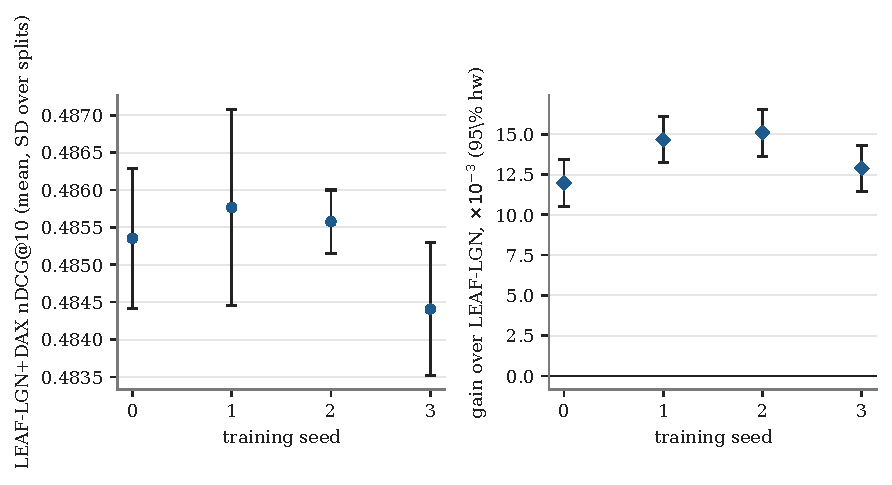
\includegraphics[width=0.85\linewidth]{figs/fig_seeds.pdf}
\caption{Training seeds 0 to 3 on KuaiRand-27K. Left: LEAF-LGN+DAX mean nDCG@10 with the standard deviation over splits, on an axis from 0.45 to 0.50. Right:
within-seed gain over LEAF-LGN, in units of $10^{-3}$, with the 95\% half-width.}
\label{fig:seeds}
\end{figure}

\end{document}
